\documentclass[twoside]{book}

% Packages required by doxygen
\usepackage{fixltx2e}
\usepackage{calc}
\usepackage{doxygen}
\usepackage[export]{adjustbox} % also loads graphicx
\usepackage{graphicx}
\usepackage[utf8]{inputenc}
\usepackage{makeidx}
\usepackage{multicol}
\usepackage{multirow}
\PassOptionsToPackage{warn}{textcomp}
\usepackage{textcomp}
\usepackage[nointegrals]{wasysym}
\usepackage[table]{xcolor}

% Font selection
\usepackage[T1]{fontenc}
\usepackage[scaled=.90]{helvet}
\usepackage{courier}
\usepackage{amssymb}
\usepackage{sectsty}
\renewcommand{\familydefault}{\sfdefault}
\allsectionsfont{%
  \fontseries{bc}\selectfont%
  \color{darkgray}%
}
\renewcommand{\DoxyLabelFont}{%
  \fontseries{bc}\selectfont%
  \color{darkgray}%
}
\newcommand{\+}{\discretionary{\mbox{\scriptsize$\hookleftarrow$}}{}{}}

% Page & text layout
\usepackage{geometry}
\geometry{%
  a4paper,%
  top=2.5cm,%
  bottom=2.5cm,%
  left=2.5cm,%
  right=2.5cm%
}
\tolerance=750
\hfuzz=15pt
\hbadness=750
\setlength{\emergencystretch}{15pt}
\setlength{\parindent}{0cm}
\setlength{\parskip}{3ex plus 2ex minus 2ex}
\makeatletter
\renewcommand{\paragraph}{%
  \@startsection{paragraph}{4}{0ex}{-1.0ex}{1.0ex}{%
    \normalfont\normalsize\bfseries\SS@parafont%
  }%
}
\renewcommand{\subparagraph}{%
  \@startsection{subparagraph}{5}{0ex}{-1.0ex}{1.0ex}{%
    \normalfont\normalsize\bfseries\SS@subparafont%
  }%
}
\makeatother

% Headers & footers
\usepackage{fancyhdr}
\pagestyle{fancyplain}
\fancyhead[LE]{\fancyplain{}{\bfseries\thepage}}
\fancyhead[CE]{\fancyplain{}{}}
\fancyhead[RE]{\fancyplain{}{\bfseries\leftmark}}
\fancyhead[LO]{\fancyplain{}{\bfseries\rightmark}}
\fancyhead[CO]{\fancyplain{}{}}
\fancyhead[RO]{\fancyplain{}{\bfseries\thepage}}
\fancyfoot[LE]{\fancyplain{}{}}
\fancyfoot[CE]{\fancyplain{}{}}
\fancyfoot[RE]{\fancyplain{}{\bfseries\scriptsize Generated by Doxygen }}
\fancyfoot[LO]{\fancyplain{}{\bfseries\scriptsize Generated by Doxygen }}
\fancyfoot[CO]{\fancyplain{}{}}
\fancyfoot[RO]{\fancyplain{}{}}
\renewcommand{\footrulewidth}{0.4pt}
\renewcommand{\chaptermark}[1]{%
  \markboth{#1}{}%
}
\renewcommand{\sectionmark}[1]{%
  \markright{\thesection\ #1}%
}

% Indices & bibliography
\usepackage{natbib}
\usepackage[titles]{tocloft}
\setcounter{tocdepth}{3}
\setcounter{secnumdepth}{5}
\makeindex

% Hyperlinks (required, but should be loaded last)
\usepackage{ifpdf}
\ifpdf
  \usepackage[pdftex,pagebackref=true]{hyperref}
\else
  \usepackage[ps2pdf,pagebackref=true]{hyperref}
\fi
\hypersetup{%
  colorlinks=true,%
  linkcolor=blue,%
  citecolor=blue,%
  unicode%
}

% Custom commands
\newcommand{\clearemptydoublepage}{%
  \newpage{\pagestyle{empty}\cleardoublepage}%
}

\usepackage{caption}
\captionsetup{labelsep=space,justification=centering,font={bf},singlelinecheck=off,skip=4pt,position=top}

%===== C O N T E N T S =====

\begin{document}

% Titlepage & ToC
\hypersetup{pageanchor=false,
             bookmarksnumbered=true,
             pdfencoding=unicode
            }
\pagenumbering{roman}
\begin{titlepage}
\vspace*{7cm}
\begin{center}%
{\Large Death\+Star Shooter }\\
\vspace*{1cm}
{\large Generated by Doxygen 1.8.11}\\
\end{center}
\end{titlepage}
\clearemptydoublepage
\tableofcontents
\clearemptydoublepage
\pagenumbering{arabic}
\hypersetup{pageanchor=true}

%--- Begin generated contents ---
\chapter{Class Index}
\section{Class List}
Here are the classes, structs, unions and interfaces with brief descriptions\+:\begin{DoxyCompactList}
\item\contentsline{section}{\hyperlink{struct___camera}{\+\_\+\+Camera} }{\pageref{struct___camera}}{}
\item\contentsline{section}{\hyperlink{struct___c_g_i}{\+\_\+\+C\+GI} }{\pageref{struct___c_g_i}}{}
\item\contentsline{section}{\hyperlink{struct___g_u_i}{\+\_\+\+G\+UI} \\*Gui est une structure composé de toutes les variable nécéssaire à linterface graphique }{\pageref{struct___g_u_i}}{}
\item\contentsline{section}{\hyperlink{struct___pantilt}{\+\_\+\+Pantilt} \\*Regroupe les variables liées à la pantilt }{\pageref{struct___pantilt}}{}
\item\contentsline{section}{\hyperlink{struct___patatoide}{\+\_\+\+Patatoide} }{\pageref{struct___patatoide}}{}
\item\contentsline{section}{\hyperlink{struct_camera}{Camera} \\*Structure contenant les variables liées à la caméra et au traitement des images reçues }{\pageref{struct_camera}}{}
\item\contentsline{section}{\hyperlink{struct_c_g_i}{C\+GI} \\*Structure contenant les images et effets à incorporer à l\textquotesingle{}image reçue }{\pageref{struct_c_g_i}}{}
\item\contentsline{section}{\hyperlink{classc_joystick}{c\+Joystick} }{\pageref{classc_joystick}}{}
\item\contentsline{section}{\hyperlink{structjoystick__position}{joystick\+\_\+position} }{\pageref{structjoystick__position}}{}
\item\contentsline{section}{\hyperlink{structjoystick__state}{joystick\+\_\+state} }{\pageref{structjoystick__state}}{}
\item\contentsline{section}{\hyperlink{struct_patatoide}{Patatoide} \\*Contient les informations relatives au patatoïde détecté }{\pageref{struct_patatoide}}{}
\end{DoxyCompactList}

\chapter{File Index}
\section{File List}
Here is a list of all files with brief descriptions\+:\begin{DoxyCompactList}
\item\contentsline{section}{\hyperlink{cgilib_8c}{cgilib.\+c} }{\pageref{cgilib_8c}}{}
\item\contentsline{section}{\hyperlink{cgilib_8h}{cgilib.\+h} \\*Ce fichier contient les prototypes des fonctions du fichier \hyperlink{cgilib_8c}{cgilib.\+c} }{\pageref{cgilib_8h}}{}
\item\contentsline{section}{\hyperlink{guilib_8c}{guilib.\+c} }{\pageref{guilib_8c}}{}
\item\contentsline{section}{\hyperlink{guilib_8h}{guilib.\+h} \\*Ce fichier contient les prototypes des fonctions liées à l\textquotesingle{}interface grapphique }{\pageref{guilib_8h}}{}
\item\contentsline{section}{\hyperlink{joystick_8c}{joystick.\+c} }{\pageref{joystick_8c}}{}
\item\contentsline{section}{\hyperlink{joystick_8h}{joystick.\+h} \\*Ce fichier contient les prototypes des fonctions liées au joystick }{\pageref{joystick_8h}}{}
\item\contentsline{section}{\hyperlink{mbdlib_8c}{mbdlib.\+c} }{\pageref{mbdlib_8c}}{}
\item\contentsline{section}{\hyperlink{mbdlib_8h}{mbdlib.\+h} \\*Ce fichier contient les prototypes des fonctions liées à la commande de la pantilt et de la archpro }{\pageref{mbdlib_8h}}{}
\item\contentsline{section}{\hyperlink{shooter_8c}{shooter.\+c} }{\pageref{shooter_8c}}{}
\item\contentsline{section}{\hyperlink{struct_8h}{struct.\+h} \\*Ce fichier regroupe les structures nécessaires à notre jeu }{\pageref{struct_8h}}{}
\end{DoxyCompactList}

\chapter{Class Documentation}
\hypertarget{struct___camera}{}\section{\+\_\+\+Camera Struct Reference}
\label{struct___camera}\index{\+\_\+\+Camera@{\+\_\+\+Camera}}


{\ttfamily \#include $<$struct.\+h$>$}

\subsection*{Public Attributes}
\begin{DoxyCompactItemize}
\item 
Ipl\+Image $\ast$ \hyperlink{struct___camera_acded182f5a3fc70318c5fca5b19bb9fe}{H\+SV}
\item 
Ipl\+Image $\ast$ \hyperlink{struct___camera_a07cebbf32e748bf08365cfe9e0726430}{threshed}
\item 
Ipl\+Image $\ast$ \hyperlink{struct___camera_a012f5d979064f440339281889f57a640}{frame}
\item 
Cv\+Scalar \hyperlink{struct___camera_a2fbe653d44adfd2e41d64b8ee08911f1}{lower\+Bound}
\item 
Cv\+Scalar \hyperlink{struct___camera_aba192c658e63df9203ec78a99e892d27}{higher\+Bound}
\item 
Cv\+Capture $\ast$ \hyperlink{struct___camera_a98541d23d3e26578d76145d7db507cfb}{cap}
\item 
Ipl\+Conv\+Kernel $\ast$ \hyperlink{struct___camera_a069a1733c9e85ccd40e15c392d0bb0bd}{elem}
\item 
int \hyperlink{struct___camera_a0bf89c266a3d53a2e1a016a61c931868}{cols}
\item 
int \hyperlink{struct___camera_a703a36cc8065f37869cc02c6b0e1c87f}{rows}
\item 
int \hyperlink{struct___camera_ae7658cf59eeb1a655b1ac5a536cc7dd4}{frame\+Number}
\end{DoxyCompactItemize}


\subsection{Member Data Documentation}
\index{\+\_\+\+Camera@{\+\_\+\+Camera}!cap@{cap}}
\index{cap@{cap}!\+\_\+\+Camera@{\+\_\+\+Camera}}
\subsubsection[{\texorpdfstring{cap}{cap}}]{\setlength{\rightskip}{0pt plus 5cm}Cv\+Capture$\ast$ \+\_\+\+Camera\+::cap}\hypertarget{struct___camera_a98541d23d3e26578d76145d7db507cfb}{}\label{struct___camera_a98541d23d3e26578d76145d7db507cfb}
La caméra d\textquotesingle{}où on récupère nos images. \index{\+\_\+\+Camera@{\+\_\+\+Camera}!cols@{cols}}
\index{cols@{cols}!\+\_\+\+Camera@{\+\_\+\+Camera}}
\subsubsection[{\texorpdfstring{cols}{cols}}]{\setlength{\rightskip}{0pt plus 5cm}int \+\_\+\+Camera\+::cols}\hypertarget{struct___camera_a0bf89c266a3d53a2e1a016a61c931868}{}\label{struct___camera_a0bf89c266a3d53a2e1a016a61c931868}
\index{\+\_\+\+Camera@{\+\_\+\+Camera}!elem@{elem}}
\index{elem@{elem}!\+\_\+\+Camera@{\+\_\+\+Camera}}
\subsubsection[{\texorpdfstring{elem}{elem}}]{\setlength{\rightskip}{0pt plus 5cm}Ipl\+Conv\+Kernel$\ast$ \+\_\+\+Camera\+::elem}\hypertarget{struct___camera_a069a1733c9e85ccd40e15c392d0bb0bd}{}\label{struct___camera_a069a1733c9e85ccd40e15c392d0bb0bd}
Element pour l\textquotesingle{}érosion. \index{\+\_\+\+Camera@{\+\_\+\+Camera}!frame@{frame}}
\index{frame@{frame}!\+\_\+\+Camera@{\+\_\+\+Camera}}
\subsubsection[{\texorpdfstring{frame}{frame}}]{\setlength{\rightskip}{0pt plus 5cm}Ipl\+Image$\ast$ \+\_\+\+Camera\+::frame}\hypertarget{struct___camera_a012f5d979064f440339281889f57a640}{}\label{struct___camera_a012f5d979064f440339281889f57a640}
Image reçue. \index{\+\_\+\+Camera@{\+\_\+\+Camera}!frame\+Number@{frame\+Number}}
\index{frame\+Number@{frame\+Number}!\+\_\+\+Camera@{\+\_\+\+Camera}}
\subsubsection[{\texorpdfstring{frame\+Number}{frameNumber}}]{\setlength{\rightskip}{0pt plus 5cm}int \+\_\+\+Camera\+::frame\+Number}\hypertarget{struct___camera_ae7658cf59eeb1a655b1ac5a536cc7dd4}{}\label{struct___camera_ae7658cf59eeb1a655b1ac5a536cc7dd4}
Donne la frame actuelle pour le déplacement des lasers. \index{\+\_\+\+Camera@{\+\_\+\+Camera}!higher\+Bound@{higher\+Bound}}
\index{higher\+Bound@{higher\+Bound}!\+\_\+\+Camera@{\+\_\+\+Camera}}
\subsubsection[{\texorpdfstring{higher\+Bound}{higherBound}}]{\setlength{\rightskip}{0pt plus 5cm}Cv\+Scalar \+\_\+\+Camera\+::higher\+Bound}\hypertarget{struct___camera_aba192c658e63df9203ec78a99e892d27}{}\label{struct___camera_aba192c658e63df9203ec78a99e892d27}
Bornes de binarisation de l\textquotesingle{}image H\+SV. \index{\+\_\+\+Camera@{\+\_\+\+Camera}!H\+SV@{H\+SV}}
\index{H\+SV@{H\+SV}!\+\_\+\+Camera@{\+\_\+\+Camera}}
\subsubsection[{\texorpdfstring{H\+SV}{HSV}}]{\setlength{\rightskip}{0pt plus 5cm}Ipl\+Image$\ast$ \+\_\+\+Camera\+::\+H\+SV}\hypertarget{struct___camera_acded182f5a3fc70318c5fca5b19bb9fe}{}\label{struct___camera_acded182f5a3fc70318c5fca5b19bb9fe}
Image reçue passée dans l\textquotesingle{}espace H\+SV. \index{\+\_\+\+Camera@{\+\_\+\+Camera}!lower\+Bound@{lower\+Bound}}
\index{lower\+Bound@{lower\+Bound}!\+\_\+\+Camera@{\+\_\+\+Camera}}
\subsubsection[{\texorpdfstring{lower\+Bound}{lowerBound}}]{\setlength{\rightskip}{0pt plus 5cm}Cv\+Scalar \+\_\+\+Camera\+::lower\+Bound}\hypertarget{struct___camera_a2fbe653d44adfd2e41d64b8ee08911f1}{}\label{struct___camera_a2fbe653d44adfd2e41d64b8ee08911f1}
\index{\+\_\+\+Camera@{\+\_\+\+Camera}!rows@{rows}}
\index{rows@{rows}!\+\_\+\+Camera@{\+\_\+\+Camera}}
\subsubsection[{\texorpdfstring{rows}{rows}}]{\setlength{\rightskip}{0pt plus 5cm}int \+\_\+\+Camera\+::rows}\hypertarget{struct___camera_a703a36cc8065f37869cc02c6b0e1c87f}{}\label{struct___camera_a703a36cc8065f37869cc02c6b0e1c87f}
Nombres de colonnes et de lignes de l\textquotesingle{}image. \index{\+\_\+\+Camera@{\+\_\+\+Camera}!threshed@{threshed}}
\index{threshed@{threshed}!\+\_\+\+Camera@{\+\_\+\+Camera}}
\subsubsection[{\texorpdfstring{threshed}{threshed}}]{\setlength{\rightskip}{0pt plus 5cm}Ipl\+Image$\ast$ \+\_\+\+Camera\+::threshed}\hypertarget{struct___camera_a07cebbf32e748bf08365cfe9e0726430}{}\label{struct___camera_a07cebbf32e748bf08365cfe9e0726430}
Image reçue binarisée depuis l\textquotesingle{}espace H\+SV. 

The documentation for this struct was generated from the following file\+:\begin{DoxyCompactItemize}
\item 
\hyperlink{struct_8h}{struct.\+h}\end{DoxyCompactItemize}

\hypertarget{struct___c_g_i}{}\section{\+\_\+\+C\+GI Struct Reference}
\label{struct___c_g_i}\index{\+\_\+\+C\+GI@{\+\_\+\+C\+GI}}


{\ttfamily \#include $<$struct.\+h$>$}

\subsection*{Public Attributes}
\begin{DoxyCompactItemize}
\item 
Ipl\+Image $\ast$ \hyperlink{struct___c_g_i_aa1d4c570026afbeb752de156cb115353}{Death\+Star}
\item 
Ipl\+Image $\ast$ \hyperlink{struct___c_g_i_a011dd009bdd05e19be0de580375359f3}{mask\+\_\+\+Death\+Star}
\item 
Ipl\+Image $\ast$ \hyperlink{struct___c_g_i_af452815aee153641ee47cd414ff40084}{Death\+Star\+\_\+resized}
\item 
Ipl\+Image $\ast$ \hyperlink{struct___c_g_i_ae6c60f83ec0f3b929305b4264928fc79}{Cockpit}
\item 
Ipl\+Image $\ast$ \hyperlink{struct___c_g_i_abdbc066c115db2c77957e1b1cd51a996}{mask\+\_\+\+Cockpit}
\item 
Cv\+Scalar \hyperlink{struct___c_g_i_a60c70aa60004326fe459e59d4e3aff5f}{mask\+Lower\+Bound}
\item 
Cv\+Scalar \hyperlink{struct___c_g_i_a7f03cda71a036dd30d70e957feee7a1c}{mask\+Higher\+Bound}
\item 
Ipl\+Image $\ast$ \hyperlink{struct___c_g_i_a8512e1bcfb9f357ebad1faf094229032}{Explosion}
\item 
Ipl\+Image $\ast$ \hyperlink{struct___c_g_i_ab35e9d17dbad69caeecb0d0eb448870c}{Explosion\+\_\+resized}
\item 
Ipl\+Image $\ast$ \hyperlink{struct___c_g_i_ae134831216d4e19fd26f578b5e720066}{mask\+\_\+\+Explosion}
\end{DoxyCompactItemize}


\subsection{Member Data Documentation}
\index{\+\_\+\+C\+GI@{\+\_\+\+C\+GI}!Cockpit@{Cockpit}}
\index{Cockpit@{Cockpit}!\+\_\+\+C\+GI@{\+\_\+\+C\+GI}}
\subsubsection[{\texorpdfstring{Cockpit}{Cockpit}}]{\setlength{\rightskip}{0pt plus 5cm}Ipl\+Image$\ast$ \+\_\+\+C\+G\+I\+::\+Cockpit}\hypertarget{struct___c_g_i_ae6c60f83ec0f3b929305b4264928fc79}{}\label{struct___c_g_i_ae6c60f83ec0f3b929305b4264928fc79}
Image du cockpit choisi. \index{\+\_\+\+C\+GI@{\+\_\+\+C\+GI}!Death\+Star@{Death\+Star}}
\index{Death\+Star@{Death\+Star}!\+\_\+\+C\+GI@{\+\_\+\+C\+GI}}
\subsubsection[{\texorpdfstring{Death\+Star}{DeathStar}}]{\setlength{\rightskip}{0pt plus 5cm}Ipl\+Image$\ast$ \+\_\+\+C\+G\+I\+::\+Death\+Star}\hypertarget{struct___c_g_i_aa1d4c570026afbeb752de156cb115353}{}\label{struct___c_g_i_aa1d4c570026afbeb752de156cb115353}
Image de l\textquotesingle{}étoile de la mort à sa taille initiale. \index{\+\_\+\+C\+GI@{\+\_\+\+C\+GI}!Death\+Star\+\_\+resized@{Death\+Star\+\_\+resized}}
\index{Death\+Star\+\_\+resized@{Death\+Star\+\_\+resized}!\+\_\+\+C\+GI@{\+\_\+\+C\+GI}}
\subsubsection[{\texorpdfstring{Death\+Star\+\_\+resized}{DeathStar_resized}}]{\setlength{\rightskip}{0pt plus 5cm}Ipl\+Image$\ast$ \+\_\+\+C\+G\+I\+::\+Death\+Star\+\_\+resized}\hypertarget{struct___c_g_i_af452815aee153641ee47cd414ff40084}{}\label{struct___c_g_i_af452815aee153641ee47cd414ff40084}
Image de l\textquotesingle{}étoile de la mort redimensionnée. \index{\+\_\+\+C\+GI@{\+\_\+\+C\+GI}!Explosion@{Explosion}}
\index{Explosion@{Explosion}!\+\_\+\+C\+GI@{\+\_\+\+C\+GI}}
\subsubsection[{\texorpdfstring{Explosion}{Explosion}}]{\setlength{\rightskip}{0pt plus 5cm}Ipl\+Image$\ast$ \+\_\+\+C\+G\+I\+::\+Explosion}\hypertarget{struct___c_g_i_a8512e1bcfb9f357ebad1faf094229032}{}\label{struct___c_g_i_a8512e1bcfb9f357ebad1faf094229032}
Image contenant l\textquotesingle{}explosion à taille initiale. \index{\+\_\+\+C\+GI@{\+\_\+\+C\+GI}!Explosion\+\_\+resized@{Explosion\+\_\+resized}}
\index{Explosion\+\_\+resized@{Explosion\+\_\+resized}!\+\_\+\+C\+GI@{\+\_\+\+C\+GI}}
\subsubsection[{\texorpdfstring{Explosion\+\_\+resized}{Explosion_resized}}]{\setlength{\rightskip}{0pt plus 5cm}Ipl\+Image$\ast$ \+\_\+\+C\+G\+I\+::\+Explosion\+\_\+resized}\hypertarget{struct___c_g_i_ab35e9d17dbad69caeecb0d0eb448870c}{}\label{struct___c_g_i_ab35e9d17dbad69caeecb0d0eb448870c}
Image contenant l\textquotesingle{}explosion redimensionnée. \index{\+\_\+\+C\+GI@{\+\_\+\+C\+GI}!mask\+\_\+\+Cockpit@{mask\+\_\+\+Cockpit}}
\index{mask\+\_\+\+Cockpit@{mask\+\_\+\+Cockpit}!\+\_\+\+C\+GI@{\+\_\+\+C\+GI}}
\subsubsection[{\texorpdfstring{mask\+\_\+\+Cockpit}{mask_Cockpit}}]{\setlength{\rightskip}{0pt plus 5cm}Ipl\+Image$\ast$ \+\_\+\+C\+G\+I\+::mask\+\_\+\+Cockpit}\hypertarget{struct___c_g_i_abdbc066c115db2c77957e1b1cd51a996}{}\label{struct___c_g_i_abdbc066c115db2c77957e1b1cd51a996}
Mask à appliquer au cockpit pour avoir une image sans fond. \index{\+\_\+\+C\+GI@{\+\_\+\+C\+GI}!mask\+\_\+\+Death\+Star@{mask\+\_\+\+Death\+Star}}
\index{mask\+\_\+\+Death\+Star@{mask\+\_\+\+Death\+Star}!\+\_\+\+C\+GI@{\+\_\+\+C\+GI}}
\subsubsection[{\texorpdfstring{mask\+\_\+\+Death\+Star}{mask_DeathStar}}]{\setlength{\rightskip}{0pt plus 5cm}Ipl\+Image$\ast$ \+\_\+\+C\+G\+I\+::mask\+\_\+\+Death\+Star}\hypertarget{struct___c_g_i_a011dd009bdd05e19be0de580375359f3}{}\label{struct___c_g_i_a011dd009bdd05e19be0de580375359f3}
Mask à appliquer à l\textquotesingle{}étoile de la mort pour avoir une image sans fond. \index{\+\_\+\+C\+GI@{\+\_\+\+C\+GI}!mask\+\_\+\+Explosion@{mask\+\_\+\+Explosion}}
\index{mask\+\_\+\+Explosion@{mask\+\_\+\+Explosion}!\+\_\+\+C\+GI@{\+\_\+\+C\+GI}}
\subsubsection[{\texorpdfstring{mask\+\_\+\+Explosion}{mask_Explosion}}]{\setlength{\rightskip}{0pt plus 5cm}Ipl\+Image$\ast$ \+\_\+\+C\+G\+I\+::mask\+\_\+\+Explosion}\hypertarget{struct___c_g_i_ae134831216d4e19fd26f578b5e720066}{}\label{struct___c_g_i_ae134831216d4e19fd26f578b5e720066}
Mask à appliquer à l\textquotesingle{}explosion pour avoir une image sans fond. \index{\+\_\+\+C\+GI@{\+\_\+\+C\+GI}!mask\+Higher\+Bound@{mask\+Higher\+Bound}}
\index{mask\+Higher\+Bound@{mask\+Higher\+Bound}!\+\_\+\+C\+GI@{\+\_\+\+C\+GI}}
\subsubsection[{\texorpdfstring{mask\+Higher\+Bound}{maskHigherBound}}]{\setlength{\rightskip}{0pt plus 5cm}Cv\+Scalar \+\_\+\+C\+G\+I\+::mask\+Higher\+Bound}\hypertarget{struct___c_g_i_a7f03cda71a036dd30d70e957feee7a1c}{}\label{struct___c_g_i_a7f03cda71a036dd30d70e957feee7a1c}
Bornes permettant l\textquotesingle{}application du mask. \index{\+\_\+\+C\+GI@{\+\_\+\+C\+GI}!mask\+Lower\+Bound@{mask\+Lower\+Bound}}
\index{mask\+Lower\+Bound@{mask\+Lower\+Bound}!\+\_\+\+C\+GI@{\+\_\+\+C\+GI}}
\subsubsection[{\texorpdfstring{mask\+Lower\+Bound}{maskLowerBound}}]{\setlength{\rightskip}{0pt plus 5cm}Cv\+Scalar \+\_\+\+C\+G\+I\+::mask\+Lower\+Bound}\hypertarget{struct___c_g_i_a60c70aa60004326fe459e59d4e3aff5f}{}\label{struct___c_g_i_a60c70aa60004326fe459e59d4e3aff5f}


The documentation for this struct was generated from the following file\+:\begin{DoxyCompactItemize}
\item 
\hyperlink{struct_8h}{struct.\+h}\end{DoxyCompactItemize}

\hypertarget{struct___g_u_i}{}\section{\+\_\+\+G\+UI Struct Reference}
\label{struct___g_u_i}\index{\+\_\+\+G\+UI@{\+\_\+\+G\+UI}}


Gui est une structure composé de toutes les variable nécéssaire à linterface graphique.  




{\ttfamily \#include $<$struct.\+h$>$}

\subsection*{Public Attributes}
\begin{DoxyCompactItemize}
\item 
Render\+Window \hyperlink{struct___g_u_i_a7466f3e309fdfed204b5b0131506f0fb}{window}
\item 
Texture \hyperlink{struct___g_u_i_a9d68467300f6039050af8f2950cc8021}{texture\+Button}
\item 
Texture \hyperlink{struct___g_u_i_a4cf2c74cbae665b04f9663c001994996}{texture\+Star\+Ship} \mbox{[}3\mbox{]}
\item 
Texture \hyperlink{struct___g_u_i_a57be58f1d814a11dc84161cc2a485d68}{texture\+Images}
\item 
Sprite \hyperlink{struct___g_u_i_a3ad6a016469abb960aca20f8dfa8ef30}{buttons} \mbox{[}3\mbox{]}
\item 
Sprite \hyperlink{struct___g_u_i_a6ff2172df7d8b7729200ea24148110a1}{sprites\+Starship} \mbox{[}3\mbox{]}
\item 
Font \hyperlink{struct___g_u_i_a57e7251e818576e9b17dd162f680d535}{font}
\item 
Text \hyperlink{struct___g_u_i_a9eb208efe8d282d8e894d1a470913091}{labels} \mbox{[}3\mbox{]}
\item 
Text \hyperlink{struct___g_u_i_ac071b81e22679f8a23e323288a3b83d5}{lab\+Title}
\item 
float \hyperlink{struct___g_u_i_aa43c86faaad13f5f449b1dca0cbd5284}{selected}
\item 
int \hyperlink{struct___g_u_i_a8c72fa2b601a788e3e182eb2f88c8787}{display}
\item 
int \hyperlink{struct___g_u_i_a00234ae245e91bfcdc4997cbfd8d275d}{starship}
\item 
unsigned char \hyperlink{struct___g_u_i_a67e0559e0707a7f3aa71f40c7ce55588}{pixels} \mbox{[}\hyperlink{struct_8h_a649b8f01fd6c0f47ff3cbddaeba63bfb}{W} $\ast$\hyperlink{struct_8h_abec92cc72a096640b821b8cd56a02495}{H} $\ast$4\mbox{]}
\end{DoxyCompactItemize}


\subsection{Detailed Description}
Gui est une structure composé de toutes les variable nécéssaire à linterface graphique. 

\subsection{Member Data Documentation}
\index{\+\_\+\+G\+UI@{\+\_\+\+G\+UI}!buttons@{buttons}}
\index{buttons@{buttons}!\+\_\+\+G\+UI@{\+\_\+\+G\+UI}}
\subsubsection[{\texorpdfstring{buttons}{buttons}}]{\setlength{\rightskip}{0pt plus 5cm}Sprite \+\_\+\+G\+U\+I\+::buttons\mbox{[}3\mbox{]}}\hypertarget{struct___g_u_i_a3ad6a016469abb960aca20f8dfa8ef30}{}\label{struct___g_u_i_a3ad6a016469abb960aca20f8dfa8ef30}
The buttons of the G\+UI \index{\+\_\+\+G\+UI@{\+\_\+\+G\+UI}!display@{display}}
\index{display@{display}!\+\_\+\+G\+UI@{\+\_\+\+G\+UI}}
\subsubsection[{\texorpdfstring{display}{display}}]{\setlength{\rightskip}{0pt plus 5cm}int \+\_\+\+G\+U\+I\+::display}\hypertarget{struct___g_u_i_a8c72fa2b601a788e3e182eb2f88c8787}{}\label{struct___g_u_i_a8c72fa2b601a788e3e182eb2f88c8787}
\index{\+\_\+\+G\+UI@{\+\_\+\+G\+UI}!font@{font}}
\index{font@{font}!\+\_\+\+G\+UI@{\+\_\+\+G\+UI}}
\subsubsection[{\texorpdfstring{font}{font}}]{\setlength{\rightskip}{0pt plus 5cm}Font \+\_\+\+G\+U\+I\+::font}\hypertarget{struct___g_u_i_a57e7251e818576e9b17dd162f680d535}{}\label{struct___g_u_i_a57e7251e818576e9b17dd162f680d535}
The font used in the gui \index{\+\_\+\+G\+UI@{\+\_\+\+G\+UI}!labels@{labels}}
\index{labels@{labels}!\+\_\+\+G\+UI@{\+\_\+\+G\+UI}}
\subsubsection[{\texorpdfstring{labels}{labels}}]{\setlength{\rightskip}{0pt plus 5cm}Text \+\_\+\+G\+U\+I\+::labels\mbox{[}3\mbox{]}}\hypertarget{struct___g_u_i_a9eb208efe8d282d8e894d1a470913091}{}\label{struct___g_u_i_a9eb208efe8d282d8e894d1a470913091}
\index{\+\_\+\+G\+UI@{\+\_\+\+G\+UI}!lab\+Title@{lab\+Title}}
\index{lab\+Title@{lab\+Title}!\+\_\+\+G\+UI@{\+\_\+\+G\+UI}}
\subsubsection[{\texorpdfstring{lab\+Title}{labTitle}}]{\setlength{\rightskip}{0pt plus 5cm}Text \+\_\+\+G\+U\+I\+::lab\+Title}\hypertarget{struct___g_u_i_ac071b81e22679f8a23e323288a3b83d5}{}\label{struct___g_u_i_ac071b81e22679f8a23e323288a3b83d5}
The \index{\+\_\+\+G\+UI@{\+\_\+\+G\+UI}!pixels@{pixels}}
\index{pixels@{pixels}!\+\_\+\+G\+UI@{\+\_\+\+G\+UI}}
\subsubsection[{\texorpdfstring{pixels}{pixels}}]{\setlength{\rightskip}{0pt plus 5cm}unsigned char \+\_\+\+G\+U\+I\+::pixels\mbox{[}{\bf W} $\ast${\bf H} $\ast$4\mbox{]}}\hypertarget{struct___g_u_i_a67e0559e0707a7f3aa71f40c7ce55588}{}\label{struct___g_u_i_a67e0559e0707a7f3aa71f40c7ce55588}
\index{\+\_\+\+G\+UI@{\+\_\+\+G\+UI}!selected@{selected}}
\index{selected@{selected}!\+\_\+\+G\+UI@{\+\_\+\+G\+UI}}
\subsubsection[{\texorpdfstring{selected}{selected}}]{\setlength{\rightskip}{0pt plus 5cm}float \+\_\+\+G\+U\+I\+::selected}\hypertarget{struct___g_u_i_aa43c86faaad13f5f449b1dca0cbd5284}{}\label{struct___g_u_i_aa43c86faaad13f5f449b1dca0cbd5284}
\index{\+\_\+\+G\+UI@{\+\_\+\+G\+UI}!sprites\+Starship@{sprites\+Starship}}
\index{sprites\+Starship@{sprites\+Starship}!\+\_\+\+G\+UI@{\+\_\+\+G\+UI}}
\subsubsection[{\texorpdfstring{sprites\+Starship}{spritesStarship}}]{\setlength{\rightskip}{0pt plus 5cm}Sprite \+\_\+\+G\+U\+I\+::sprites\+Starship\mbox{[}3\mbox{]}}\hypertarget{struct___g_u_i_a6ff2172df7d8b7729200ea24148110a1}{}\label{struct___g_u_i_a6ff2172df7d8b7729200ea24148110a1}
The buttons of the G\+UI \index{\+\_\+\+G\+UI@{\+\_\+\+G\+UI}!starship@{starship}}
\index{starship@{starship}!\+\_\+\+G\+UI@{\+\_\+\+G\+UI}}
\subsubsection[{\texorpdfstring{starship}{starship}}]{\setlength{\rightskip}{0pt plus 5cm}int \+\_\+\+G\+U\+I\+::starship}\hypertarget{struct___g_u_i_a00234ae245e91bfcdc4997cbfd8d275d}{}\label{struct___g_u_i_a00234ae245e91bfcdc4997cbfd8d275d}
\index{\+\_\+\+G\+UI@{\+\_\+\+G\+UI}!texture\+Button@{texture\+Button}}
\index{texture\+Button@{texture\+Button}!\+\_\+\+G\+UI@{\+\_\+\+G\+UI}}
\subsubsection[{\texorpdfstring{texture\+Button}{textureButton}}]{\setlength{\rightskip}{0pt plus 5cm}Texture \+\_\+\+G\+U\+I\+::texture\+Button}\hypertarget{struct___g_u_i_a9d68467300f6039050af8f2950cc8021}{}\label{struct___g_u_i_a9d68467300f6039050af8f2950cc8021}
\index{\+\_\+\+G\+UI@{\+\_\+\+G\+UI}!texture\+Images@{texture\+Images}}
\index{texture\+Images@{texture\+Images}!\+\_\+\+G\+UI@{\+\_\+\+G\+UI}}
\subsubsection[{\texorpdfstring{texture\+Images}{textureImages}}]{\setlength{\rightskip}{0pt plus 5cm}Texture \+\_\+\+G\+U\+I\+::texture\+Images}\hypertarget{struct___g_u_i_a57be58f1d814a11dc84161cc2a485d68}{}\label{struct___g_u_i_a57be58f1d814a11dc84161cc2a485d68}
texture of the differents gui objects \index{\+\_\+\+G\+UI@{\+\_\+\+G\+UI}!texture\+Star\+Ship@{texture\+Star\+Ship}}
\index{texture\+Star\+Ship@{texture\+Star\+Ship}!\+\_\+\+G\+UI@{\+\_\+\+G\+UI}}
\subsubsection[{\texorpdfstring{texture\+Star\+Ship}{textureStarShip}}]{\setlength{\rightskip}{0pt plus 5cm}Texture \+\_\+\+G\+U\+I\+::texture\+Star\+Ship\mbox{[}3\mbox{]}}\hypertarget{struct___g_u_i_a4cf2c74cbae665b04f9663c001994996}{}\label{struct___g_u_i_a4cf2c74cbae665b04f9663c001994996}
\index{\+\_\+\+G\+UI@{\+\_\+\+G\+UI}!window@{window}}
\index{window@{window}!\+\_\+\+G\+UI@{\+\_\+\+G\+UI}}
\subsubsection[{\texorpdfstring{window}{window}}]{\setlength{\rightskip}{0pt plus 5cm}Render\+Window \+\_\+\+G\+U\+I\+::window}\hypertarget{struct___g_u_i_a7466f3e309fdfed204b5b0131506f0fb}{}\label{struct___g_u_i_a7466f3e309fdfed204b5b0131506f0fb}
The window 

The documentation for this struct was generated from the following file\+:\begin{DoxyCompactItemize}
\item 
\hyperlink{struct_8h}{struct.\+h}\end{DoxyCompactItemize}

\hypertarget{struct___pantilt}{}\section{\+\_\+\+Pantilt Struct Reference}
\label{struct___pantilt}\index{\+\_\+\+Pantilt@{\+\_\+\+Pantilt}}


Regroupe les variables liées à la pantilt.  




{\ttfamily \#include $<$struct.\+h$>$}

\subsection*{Public Attributes}
\begin{DoxyCompactItemize}
\item 
float \hyperlink{struct___pantilt_a176de6650a3e2cd0b1a368341113c6be}{pos\+M1}
\item 
float \hyperlink{struct___pantilt_a3db337f00d74f2f7d2d4a566fa752864}{pos\+M2}
\item 
int \hyperlink{struct___pantilt_adf84d6bc2232f3b4bc0f083ba9fb7d6e}{min\+M1}
\item 
int \hyperlink{struct___pantilt_a7a297f4584b4716b650e36bd7b52b933}{max\+M1}
\item 
int \hyperlink{struct___pantilt_a699ffbddf43d385ee176a11ed0824483}{min\+M2}
\item 
int \hyperlink{struct___pantilt_a3d40173704b6bee3917c36ad86e4d506}{max\+M2}
\item 
float \hyperlink{struct___pantilt_a8cdf704a9fb3b595305ec85fa3b6c0e6}{ease}
\item 
int \hyperlink{struct___pantilt_ad01a4e572846f68131a375e708a825aa}{arch\+Pro}
\item 
char \hyperlink{struct___pantilt_aa3d78142802cbd9374bc905f81539a37}{buffer} \mbox{[}64\mbox{]}
\item 
char \hyperlink{struct___pantilt_ac1ef92bf2930646a3950cbe0b426b30d}{str} \mbox{[}8\mbox{]}
\end{DoxyCompactItemize}


\subsection{Detailed Description}
Regroupe les variables liées à la pantilt. 

\subsection{Member Data Documentation}
\index{\+\_\+\+Pantilt@{\+\_\+\+Pantilt}!arch\+Pro@{arch\+Pro}}
\index{arch\+Pro@{arch\+Pro}!\+\_\+\+Pantilt@{\+\_\+\+Pantilt}}
\subsubsection[{\texorpdfstring{arch\+Pro}{archPro}}]{\setlength{\rightskip}{0pt plus 5cm}int \+\_\+\+Pantilt\+::arch\+Pro}\hypertarget{struct___pantilt_ad01a4e572846f68131a375e708a825aa}{}\label{struct___pantilt_ad01a4e572846f68131a375e708a825aa}
File descriptor of the embed microcontroller \index{\+\_\+\+Pantilt@{\+\_\+\+Pantilt}!buffer@{buffer}}
\index{buffer@{buffer}!\+\_\+\+Pantilt@{\+\_\+\+Pantilt}}
\subsubsection[{\texorpdfstring{buffer}{buffer}}]{\setlength{\rightskip}{0pt plus 5cm}char \+\_\+\+Pantilt\+::buffer\mbox{[}64\mbox{]}}\hypertarget{struct___pantilt_aa3d78142802cbd9374bc905f81539a37}{}\label{struct___pantilt_aa3d78142802cbd9374bc905f81539a37}
\index{\+\_\+\+Pantilt@{\+\_\+\+Pantilt}!ease@{ease}}
\index{ease@{ease}!\+\_\+\+Pantilt@{\+\_\+\+Pantilt}}
\subsubsection[{\texorpdfstring{ease}{ease}}]{\setlength{\rightskip}{0pt plus 5cm}float \+\_\+\+Pantilt\+::ease}\hypertarget{struct___pantilt_a8cdf704a9fb3b595305ec85fa3b6c0e6}{}\label{struct___pantilt_a8cdf704a9fb3b595305ec85fa3b6c0e6}
Coeficient to filter the position command of the motors. \index{\+\_\+\+Pantilt@{\+\_\+\+Pantilt}!max\+M1@{max\+M1}}
\index{max\+M1@{max\+M1}!\+\_\+\+Pantilt@{\+\_\+\+Pantilt}}
\subsubsection[{\texorpdfstring{max\+M1}{maxM1}}]{\setlength{\rightskip}{0pt plus 5cm}int \+\_\+\+Pantilt\+::max\+M1}\hypertarget{struct___pantilt_a7a297f4584b4716b650e36bd7b52b933}{}\label{struct___pantilt_a7a297f4584b4716b650e36bd7b52b933}
Maximums positions of the motor 1. \index{\+\_\+\+Pantilt@{\+\_\+\+Pantilt}!max\+M2@{max\+M2}}
\index{max\+M2@{max\+M2}!\+\_\+\+Pantilt@{\+\_\+\+Pantilt}}
\subsubsection[{\texorpdfstring{max\+M2}{maxM2}}]{\setlength{\rightskip}{0pt plus 5cm}int \+\_\+\+Pantilt\+::max\+M2}\hypertarget{struct___pantilt_a3d40173704b6bee3917c36ad86e4d506}{}\label{struct___pantilt_a3d40173704b6bee3917c36ad86e4d506}
Maximums positions of the motor 1. \index{\+\_\+\+Pantilt@{\+\_\+\+Pantilt}!min\+M1@{min\+M1}}
\index{min\+M1@{min\+M1}!\+\_\+\+Pantilt@{\+\_\+\+Pantilt}}
\subsubsection[{\texorpdfstring{min\+M1}{minM1}}]{\setlength{\rightskip}{0pt plus 5cm}int \+\_\+\+Pantilt\+::min\+M1}\hypertarget{struct___pantilt_adf84d6bc2232f3b4bc0f083ba9fb7d6e}{}\label{struct___pantilt_adf84d6bc2232f3b4bc0f083ba9fb7d6e}
\index{\+\_\+\+Pantilt@{\+\_\+\+Pantilt}!min\+M2@{min\+M2}}
\index{min\+M2@{min\+M2}!\+\_\+\+Pantilt@{\+\_\+\+Pantilt}}
\subsubsection[{\texorpdfstring{min\+M2}{minM2}}]{\setlength{\rightskip}{0pt plus 5cm}int \+\_\+\+Pantilt\+::min\+M2}\hypertarget{struct___pantilt_a699ffbddf43d385ee176a11ed0824483}{}\label{struct___pantilt_a699ffbddf43d385ee176a11ed0824483}
\index{\+\_\+\+Pantilt@{\+\_\+\+Pantilt}!pos\+M1@{pos\+M1}}
\index{pos\+M1@{pos\+M1}!\+\_\+\+Pantilt@{\+\_\+\+Pantilt}}
\subsubsection[{\texorpdfstring{pos\+M1}{posM1}}]{\setlength{\rightskip}{0pt plus 5cm}float \+\_\+\+Pantilt\+::pos\+M1}\hypertarget{struct___pantilt_a176de6650a3e2cd0b1a368341113c6be}{}\label{struct___pantilt_a176de6650a3e2cd0b1a368341113c6be}
\index{\+\_\+\+Pantilt@{\+\_\+\+Pantilt}!pos\+M2@{pos\+M2}}
\index{pos\+M2@{pos\+M2}!\+\_\+\+Pantilt@{\+\_\+\+Pantilt}}
\subsubsection[{\texorpdfstring{pos\+M2}{posM2}}]{\setlength{\rightskip}{0pt plus 5cm}float \+\_\+\+Pantilt\+::pos\+M2}\hypertarget{struct___pantilt_a3db337f00d74f2f7d2d4a566fa752864}{}\label{struct___pantilt_a3db337f00d74f2f7d2d4a566fa752864}
Current positions of the motors. \index{\+\_\+\+Pantilt@{\+\_\+\+Pantilt}!str@{str}}
\index{str@{str}!\+\_\+\+Pantilt@{\+\_\+\+Pantilt}}
\subsubsection[{\texorpdfstring{str}{str}}]{\setlength{\rightskip}{0pt plus 5cm}char \+\_\+\+Pantilt\+::str\mbox{[}8\mbox{]}}\hypertarget{struct___pantilt_ac1ef92bf2930646a3950cbe0b426b30d}{}\label{struct___pantilt_ac1ef92bf2930646a3950cbe0b426b30d}


The documentation for this struct was generated from the following file\+:\begin{DoxyCompactItemize}
\item 
\hyperlink{struct_8h}{struct.\+h}\end{DoxyCompactItemize}

\hypertarget{struct___patatoide}{}\section{\+\_\+\+Patatoide Struct Reference}
\label{struct___patatoide}\index{\+\_\+\+Patatoide@{\+\_\+\+Patatoide}}


{\ttfamily \#include $<$struct.\+h$>$}

\subsection*{Public Attributes}
\begin{DoxyCompactItemize}
\item 
Cv\+Point \hyperlink{struct___patatoide_af09e794797d7eff23275a6415334c7d3}{centre}
\item 
int \hyperlink{struct___patatoide_a3de9938e002e44bf1c395af4811dc048}{moy}
\item 
int \hyperlink{struct___patatoide_a3154bc1cd89cedada3ad78fe9f69c23d}{percentage}
\end{DoxyCompactItemize}


\subsection{Member Data Documentation}
\index{\+\_\+\+Patatoide@{\+\_\+\+Patatoide}!centre@{centre}}
\index{centre@{centre}!\+\_\+\+Patatoide@{\+\_\+\+Patatoide}}
\subsubsection[{\texorpdfstring{centre}{centre}}]{\setlength{\rightskip}{0pt plus 5cm}Cv\+Point \+\_\+\+Patatoide\+::centre}\hypertarget{struct___patatoide_af09e794797d7eff23275a6415334c7d3}{}\label{struct___patatoide_af09e794797d7eff23275a6415334c7d3}
Centre du patatoïde. \index{\+\_\+\+Patatoide@{\+\_\+\+Patatoide}!moy@{moy}}
\index{moy@{moy}!\+\_\+\+Patatoide@{\+\_\+\+Patatoide}}
\subsubsection[{\texorpdfstring{moy}{moy}}]{\setlength{\rightskip}{0pt plus 5cm}int \+\_\+\+Patatoide\+::moy}\hypertarget{struct___patatoide_a3de9938e002e44bf1c395af4811dc048}{}\label{struct___patatoide_a3de9938e002e44bf1c395af4811dc048}
\char`\"{}taille\char`\"{} du patatoïde en nombre de pixels, avec une évolution pondérée par un coefficient. \index{\+\_\+\+Patatoide@{\+\_\+\+Patatoide}!percentage@{percentage}}
\index{percentage@{percentage}!\+\_\+\+Patatoide@{\+\_\+\+Patatoide}}
\subsubsection[{\texorpdfstring{percentage}{percentage}}]{\setlength{\rightskip}{0pt plus 5cm}int \+\_\+\+Patatoide\+::percentage}\hypertarget{struct___patatoide_a3154bc1cd89cedada3ad78fe9f69c23d}{}\label{struct___patatoide_a3154bc1cd89cedada3ad78fe9f69c23d}
Taille du patatoide en pourcentage par rapport à l\textquotesingle{}image initiale. 

The documentation for this struct was generated from the following file\+:\begin{DoxyCompactItemize}
\item 
\hyperlink{struct_8h}{struct.\+h}\end{DoxyCompactItemize}

\hypertarget{struct_camera}{}\section{Camera Struct Reference}
\label{struct_camera}\index{Camera@{Camera}}


Structure contenant les variables liées à la caméra et au traitement des images reçues.  




{\ttfamily \#include $<$struct.\+h$>$}



\subsection{Detailed Description}
Structure contenant les variables liées à la caméra et au traitement des images reçues. 

The documentation for this struct was generated from the following file\+:\begin{DoxyCompactItemize}
\item 
\hyperlink{struct_8h}{struct.\+h}\end{DoxyCompactItemize}

\hypertarget{struct_c_g_i}{}\section{C\+GI Struct Reference}
\label{struct_c_g_i}\index{C\+GI@{C\+GI}}


Structure contenant les images et effets à incorporer à l\textquotesingle{}image reçue.  




{\ttfamily \#include $<$struct.\+h$>$}



\subsection{Detailed Description}
Structure contenant les images et effets à incorporer à l\textquotesingle{}image reçue. 

The documentation for this struct was generated from the following file\+:\begin{DoxyCompactItemize}
\item 
\hyperlink{struct_8h}{struct.\+h}\end{DoxyCompactItemize}

\hypertarget{classc_joystick}{}\section{c\+Joystick Class Reference}
\label{classc_joystick}\index{c\+Joystick@{c\+Joystick}}


{\ttfamily \#include $<$joystick.\+h$>$}

\subsection*{Public Member Functions}
\begin{DoxyCompactItemize}
\item 
\hyperlink{classc_joystick_ae4edecc3589f19b068113cdb79f7b39d}{c\+Joystick} ()
\item 
\hyperlink{classc_joystick_a9e429f765dee1dc7dc3d31dc0f50ae0e}{$\sim$c\+Joystick} ()
\item 
void \hyperlink{classc_joystick_a8c04dc903aac9588db3b3e81f495705a}{read\+Ev} ()
\item 
\hyperlink{structjoystick__position}{joystick\+\_\+position} \hyperlink{classc_joystick_a30d938005453ad77f512094c8a7a99f5}{joystick\+Position} (int n)
\item 
int \hyperlink{classc_joystick_a2954017eb51ef6f4658450199e5df5b4}{joystick\+Value} (int n)
\item 
bool \hyperlink{classc_joystick_a10375763b82c2da3e904d118d5cf2ecb}{button\+Pressed} (int n)
\end{DoxyCompactItemize}
\subsection*{Static Public Member Functions}
\begin{DoxyCompactItemize}
\item 
static void $\ast$ \hyperlink{classc_joystick_aafa52c2e4d67c71f3d1e31b80d1dd324}{loop} (void $\ast$obj)
\end{DoxyCompactItemize}


\subsection{Constructor \& Destructor Documentation}
\index{c\+Joystick@{c\+Joystick}!c\+Joystick@{c\+Joystick}}
\index{c\+Joystick@{c\+Joystick}!c\+Joystick@{c\+Joystick}}
\subsubsection[{\texorpdfstring{c\+Joystick()}{cJoystick()}}]{\setlength{\rightskip}{0pt plus 5cm}c\+Joystick\+::c\+Joystick (
\begin{DoxyParamCaption}
{}
\end{DoxyParamCaption}
)}\hypertarget{classc_joystick_ae4edecc3589f19b068113cdb79f7b39d}{}\label{classc_joystick_ae4edecc3589f19b068113cdb79f7b39d}
\index{c\+Joystick@{c\+Joystick}!````~c\+Joystick@{$\sim$c\+Joystick}}
\index{````~c\+Joystick@{$\sim$c\+Joystick}!c\+Joystick@{c\+Joystick}}
\subsubsection[{\texorpdfstring{$\sim$c\+Joystick()}{~cJoystick()}}]{\setlength{\rightskip}{0pt plus 5cm}c\+Joystick\+::$\sim$c\+Joystick (
\begin{DoxyParamCaption}
{}
\end{DoxyParamCaption}
)}\hypertarget{classc_joystick_a9e429f765dee1dc7dc3d31dc0f50ae0e}{}\label{classc_joystick_a9e429f765dee1dc7dc3d31dc0f50ae0e}


\subsection{Member Function Documentation}
\index{c\+Joystick@{c\+Joystick}!button\+Pressed@{button\+Pressed}}
\index{button\+Pressed@{button\+Pressed}!c\+Joystick@{c\+Joystick}}
\subsubsection[{\texorpdfstring{button\+Pressed(int n)}{buttonPressed(int n)}}]{\setlength{\rightskip}{0pt plus 5cm}bool c\+Joystick\+::button\+Pressed (
\begin{DoxyParamCaption}
\item[{int}]{n}
\end{DoxyParamCaption}
)}\hypertarget{classc_joystick_a10375763b82c2da3e904d118d5cf2ecb}{}\label{classc_joystick_a10375763b82c2da3e904d118d5cf2ecb}
\index{c\+Joystick@{c\+Joystick}!joystick\+Position@{joystick\+Position}}
\index{joystick\+Position@{joystick\+Position}!c\+Joystick@{c\+Joystick}}
\subsubsection[{\texorpdfstring{joystick\+Position(int n)}{joystickPosition(int n)}}]{\setlength{\rightskip}{0pt plus 5cm}{\bf joystick\+\_\+position} c\+Joystick\+::joystick\+Position (
\begin{DoxyParamCaption}
\item[{int}]{n}
\end{DoxyParamCaption}
)}\hypertarget{classc_joystick_a30d938005453ad77f512094c8a7a99f5}{}\label{classc_joystick_a30d938005453ad77f512094c8a7a99f5}
\index{c\+Joystick@{c\+Joystick}!joystick\+Value@{joystick\+Value}}
\index{joystick\+Value@{joystick\+Value}!c\+Joystick@{c\+Joystick}}
\subsubsection[{\texorpdfstring{joystick\+Value(int n)}{joystickValue(int n)}}]{\setlength{\rightskip}{0pt plus 5cm}int c\+Joystick\+::joystick\+Value (
\begin{DoxyParamCaption}
\item[{int}]{n}
\end{DoxyParamCaption}
)}\hypertarget{classc_joystick_a2954017eb51ef6f4658450199e5df5b4}{}\label{classc_joystick_a2954017eb51ef6f4658450199e5df5b4}
\index{c\+Joystick@{c\+Joystick}!loop@{loop}}
\index{loop@{loop}!c\+Joystick@{c\+Joystick}}
\subsubsection[{\texorpdfstring{loop(void $\ast$obj)}{loop(void *obj)}}]{\setlength{\rightskip}{0pt plus 5cm}void $\ast$ c\+Joystick\+::loop (
\begin{DoxyParamCaption}
\item[{void $\ast$}]{obj}
\end{DoxyParamCaption}
)\hspace{0.3cm}{\ttfamily [static]}}\hypertarget{classc_joystick_aafa52c2e4d67c71f3d1e31b80d1dd324}{}\label{classc_joystick_aafa52c2e4d67c71f3d1e31b80d1dd324}
\index{c\+Joystick@{c\+Joystick}!read\+Ev@{read\+Ev}}
\index{read\+Ev@{read\+Ev}!c\+Joystick@{c\+Joystick}}
\subsubsection[{\texorpdfstring{read\+Ev()}{readEv()}}]{\setlength{\rightskip}{0pt plus 5cm}void c\+Joystick\+::read\+Ev (
\begin{DoxyParamCaption}
{}
\end{DoxyParamCaption}
)}\hypertarget{classc_joystick_a8c04dc903aac9588db3b3e81f495705a}{}\label{classc_joystick_a8c04dc903aac9588db3b3e81f495705a}


The documentation for this class was generated from the following files\+:\begin{DoxyCompactItemize}
\item 
\hyperlink{joystick_8h}{joystick.\+h}\item 
\hyperlink{joystick_8c}{joystick.\+c}\end{DoxyCompactItemize}

\hypertarget{structjoystick__position}{}\section{joystick\+\_\+position Struct Reference}
\label{structjoystick__position}\index{joystick\+\_\+position@{joystick\+\_\+position}}


{\ttfamily \#include $<$joystick.\+h$>$}

\subsection*{Public Attributes}
\begin{DoxyCompactItemize}
\item 
float \hyperlink{structjoystick__position_ad738e8acb3656438c10d2ec7670639e5}{theta}
\item 
float \hyperlink{structjoystick__position_a0a9043868a14fce25888dd81b80f6c94}{r}
\item 
float \hyperlink{structjoystick__position_a71c3292c1be3c3400a388eac41a47ad3}{x}
\item 
float \hyperlink{structjoystick__position_ad8fc27fbd5404a4f8cdc1a045a0d689a}{y}
\end{DoxyCompactItemize}


\subsection{Member Data Documentation}
\index{joystick\+\_\+position@{joystick\+\_\+position}!r@{r}}
\index{r@{r}!joystick\+\_\+position@{joystick\+\_\+position}}
\subsubsection[{\texorpdfstring{r}{r}}]{\setlength{\rightskip}{0pt plus 5cm}float joystick\+\_\+position\+::r}\hypertarget{structjoystick__position_a0a9043868a14fce25888dd81b80f6c94}{}\label{structjoystick__position_a0a9043868a14fce25888dd81b80f6c94}
\index{joystick\+\_\+position@{joystick\+\_\+position}!theta@{theta}}
\index{theta@{theta}!joystick\+\_\+position@{joystick\+\_\+position}}
\subsubsection[{\texorpdfstring{theta}{theta}}]{\setlength{\rightskip}{0pt plus 5cm}float joystick\+\_\+position\+::theta}\hypertarget{structjoystick__position_ad738e8acb3656438c10d2ec7670639e5}{}\label{structjoystick__position_ad738e8acb3656438c10d2ec7670639e5}
\index{joystick\+\_\+position@{joystick\+\_\+position}!x@{x}}
\index{x@{x}!joystick\+\_\+position@{joystick\+\_\+position}}
\subsubsection[{\texorpdfstring{x}{x}}]{\setlength{\rightskip}{0pt plus 5cm}float joystick\+\_\+position\+::x}\hypertarget{structjoystick__position_a71c3292c1be3c3400a388eac41a47ad3}{}\label{structjoystick__position_a71c3292c1be3c3400a388eac41a47ad3}
\index{joystick\+\_\+position@{joystick\+\_\+position}!y@{y}}
\index{y@{y}!joystick\+\_\+position@{joystick\+\_\+position}}
\subsubsection[{\texorpdfstring{y}{y}}]{\setlength{\rightskip}{0pt plus 5cm}float joystick\+\_\+position\+::y}\hypertarget{structjoystick__position_ad8fc27fbd5404a4f8cdc1a045a0d689a}{}\label{structjoystick__position_ad8fc27fbd5404a4f8cdc1a045a0d689a}


The documentation for this struct was generated from the following file\+:\begin{DoxyCompactItemize}
\item 
\hyperlink{joystick_8h}{joystick.\+h}\end{DoxyCompactItemize}

\hypertarget{structjoystick__state}{}\section{joystick\+\_\+state Struct Reference}
\label{structjoystick__state}\index{joystick\+\_\+state@{joystick\+\_\+state}}


{\ttfamily \#include $<$joystick.\+h$>$}

\subsection*{Public Attributes}
\begin{DoxyCompactItemize}
\item 
std\+::vector$<$ signed short $>$ \hyperlink{structjoystick__state_af16d0e2bea842ab4fafa05ce23f45f56}{button}
\item 
std\+::vector$<$ signed short $>$ \hyperlink{structjoystick__state_acc10718083ec5603bfcca9d1780239f2}{axis}
\end{DoxyCompactItemize}


\subsection{Member Data Documentation}
\index{joystick\+\_\+state@{joystick\+\_\+state}!axis@{axis}}
\index{axis@{axis}!joystick\+\_\+state@{joystick\+\_\+state}}
\subsubsection[{\texorpdfstring{axis}{axis}}]{\setlength{\rightskip}{0pt plus 5cm}std\+::vector$<$signed short$>$ joystick\+\_\+state\+::axis}\hypertarget{structjoystick__state_acc10718083ec5603bfcca9d1780239f2}{}\label{structjoystick__state_acc10718083ec5603bfcca9d1780239f2}
\index{joystick\+\_\+state@{joystick\+\_\+state}!button@{button}}
\index{button@{button}!joystick\+\_\+state@{joystick\+\_\+state}}
\subsubsection[{\texorpdfstring{button}{button}}]{\setlength{\rightskip}{0pt plus 5cm}std\+::vector$<$signed short$>$ joystick\+\_\+state\+::button}\hypertarget{structjoystick__state_af16d0e2bea842ab4fafa05ce23f45f56}{}\label{structjoystick__state_af16d0e2bea842ab4fafa05ce23f45f56}


The documentation for this struct was generated from the following file\+:\begin{DoxyCompactItemize}
\item 
\hyperlink{joystick_8h}{joystick.\+h}\end{DoxyCompactItemize}

\hypertarget{struct_patatoide}{}\section{Patatoide Struct Reference}
\label{struct_patatoide}\index{Patatoide@{Patatoide}}


Contient les informations relatives au patatoïde détecté  




{\ttfamily \#include $<$struct.\+h$>$}



\subsection{Detailed Description}
Contient les informations relatives au patatoïde détecté 

The documentation for this struct was generated from the following file\+:\begin{DoxyCompactItemize}
\item 
\hyperlink{struct_8h}{struct.\+h}\end{DoxyCompactItemize}

\chapter{File Documentation}
\hypertarget{cgilib_8c}{}\section{cgilib.\+c File Reference}
\label{cgilib_8c}\index{cgilib.\+c@{cgilib.\+c}}
{\ttfamily \#include $<$stdio.\+h$>$}\\*
{\ttfamily \#include \char`\"{}struct.\+h\char`\"{}}\\*
Include dependency graph for cgilib.\+c\+:
\nopagebreak
\begin{figure}[H]
\begin{center}
\leavevmode
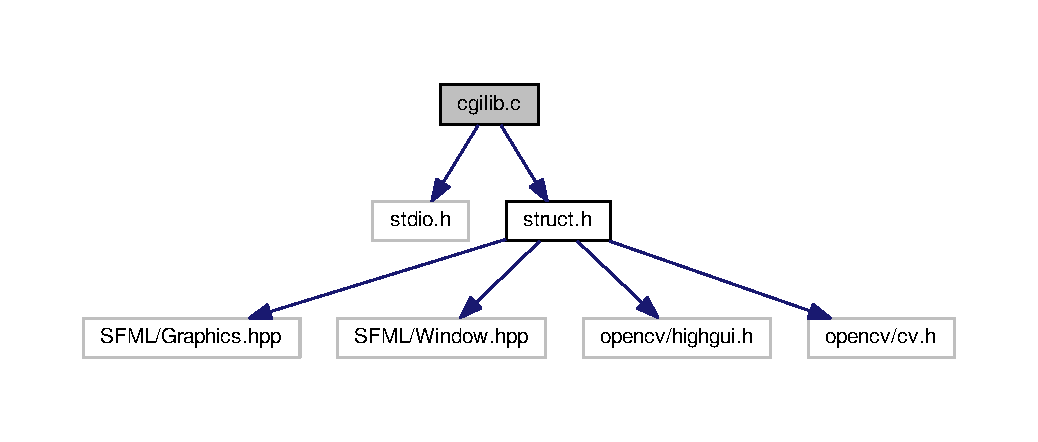
\includegraphics[width=350pt]{cgilib_8c__incl}
\end{center}
\end{figure}
\subsection*{Functions}
\begin{DoxyCompactItemize}
\item 
void \hyperlink{cgilib_8c_a59601d55e89384d9c991d0a306f28f04}{laser} (Ipl\+Image $\ast$img, int frame\+Number)
\begin{DoxyCompactList}\small\item\em Fonction d\textquotesingle{}animation des lasers sur l\textquotesingle{}image. \end{DoxyCompactList}\item 
void \hyperlink{cgilib_8c_a47a39404e5c0cdfae0165f8e3de5e3d5}{release\+\_\+final} (\hyperlink{struct_camera}{Camera} $\ast$cam, \hyperlink{struct_c_g_i}{C\+GI} $\ast$after\+Effect)
\item 
void \hyperlink{cgilib_8c_a8478b3dd0067e674a7f546f3d8a1973f}{release\+\_\+boucle} (\hyperlink{struct_c_g_i}{C\+GI} $\ast$after\+Effect, \hyperlink{struct_camera}{Camera} $\ast$cam)
\item 
Ipl\+Image $\ast$ \hyperlink{cgilib_8c_a93982521c1e437ed015d3870024378aa}{resize} (Ipl\+Image $\ast$src, int percentage)
\begin{DoxyCompactList}\small\item\em Fonction qui redimensionne une image en pourcentage de sa taille initiale. \end{DoxyCompactList}\item 
Ipl\+Image $\ast$ \hyperlink{cgilib_8c_a25a21584c96a36aba95f6d40245de59d}{init\+\_\+cockpit} (int i)
\item 
void \hyperlink{cgilib_8c_aef64f26cc8f7854b0cfcbf94efa105d1}{calcul\+\_\+patate} (\hyperlink{struct_patatoide}{Patatoide} $\ast$patate, \hyperlink{struct_camera}{Camera} $\ast$cam, float coeff)
\begin{DoxyCompactList}\small\item\em Fonction effectuant des calculs amenant à connaître le centre et la taille du patatoïde observé. \end{DoxyCompactList}\item 
void \hyperlink{cgilib_8c_a4ba7b36502846e591ed35dcfacfbfe0a}{init\+\_\+mask} (\hyperlink{struct_c_g_i}{C\+GI} $\ast$after\+Effect)
\item 
void \hyperlink{cgilib_8c_aef0ed3eef749bb66dce0408ed5c71751}{create\+\_\+mask} (\hyperlink{struct_c_g_i}{C\+GI} $\ast$after\+Effect, int mode, int w\+\_\+resized, int h\+\_\+resized)
\item 
int \hyperlink{cgilib_8c_a5423edb32e5bf81ad59c86966a7494c6}{init\+\_\+cam} (\hyperlink{struct_camera}{Camera} $\ast$cam)
\begin{DoxyCompactList}\small\item\em Fonction d\textquotesingle{}initialisation des différents paramètres liées à la caméra. \end{DoxyCompactList}\item 
void \hyperlink{cgilib_8c_a38a7d29cdb7a9f133a6845b22644e6ac}{insert\+\_\+image} (struct \hyperlink{struct___c_g_i}{\+\_\+\+C\+GI} $\ast$after\+Effect, \hyperlink{struct_camera}{Camera} $\ast$cam, \hyperlink{struct_patatoide}{Patatoide} $\ast$patate, int mode)
\begin{DoxyCompactList}\small\item\em Fonction d\textquotesingle{}insertion d\textquotesingle{}image plus petite dans l\textquotesingle{}image affichée. \end{DoxyCompactList}\item 
int \hyperlink{cgilib_8c_a731bf42d8f37ed38b2865dd7b06bb031}{is\+Touched} (\hyperlink{struct_patatoide}{Patatoide} patate)
\begin{DoxyCompactList}\small\item\em Fonction qui détermine si l\textquotesingle{}on a touché l\textquotesingle{}étoile ou non lors de notre tir. \end{DoxyCompactList}\end{DoxyCompactItemize}


\subsection{Function Documentation}
\index{cgilib.\+c@{cgilib.\+c}!calcul\+\_\+patate@{calcul\+\_\+patate}}
\index{calcul\+\_\+patate@{calcul\+\_\+patate}!cgilib.\+c@{cgilib.\+c}}
\subsubsection[{\texorpdfstring{calcul\+\_\+patate(\+Patatoide $\ast$patate, Camera $\ast$cam, float coeff)}{calcul_patate(Patatoide *patate, Camera *cam, float coeff)}}]{\setlength{\rightskip}{0pt plus 5cm}void calcul\+\_\+patate (
\begin{DoxyParamCaption}
\item[{{\bf Patatoide} $\ast$}]{patate, }
\item[{{\bf Camera} $\ast$}]{cam, }
\item[{float}]{coeff}
\end{DoxyParamCaption}
)}\hypertarget{cgilib_8c_aef64f26cc8f7854b0cfcbf94efa105d1}{}\label{cgilib_8c_aef64f26cc8f7854b0cfcbf94efa105d1}


Fonction effectuant des calculs amenant à connaître le centre et la taille du patatoïde observé. 


\begin{DoxyParams}{Parameters}
{\em patate} & Structure contenant les informations sur le patatoïde. \\
\hline
{\em cam} & Structure contenant des pointeurs sur les images utilisées dans le programme. \\
\hline
{\em coeff} & Valeur choisie à 0.\+1 ajustant la variation de la taille du patatoïde pour empêcher une évolution trop brusque. \\
\hline
\end{DoxyParams}
\begin{DoxyReturn}{Returns}
void. 
\end{DoxyReturn}
\index{cgilib.\+c@{cgilib.\+c}!create\+\_\+mask@{create\+\_\+mask}}
\index{create\+\_\+mask@{create\+\_\+mask}!cgilib.\+c@{cgilib.\+c}}
\subsubsection[{\texorpdfstring{create\+\_\+mask(\+C\+G\+I $\ast$after\+Effect, int mode, int w\+\_\+resized, int h\+\_\+resized)}{create_mask(CGI *afterEffect, int mode, int w_resized, int h_resized)}}]{\setlength{\rightskip}{0pt plus 5cm}void create\+\_\+mask (
\begin{DoxyParamCaption}
\item[{{\bf C\+GI} $\ast$}]{after\+Effect, }
\item[{int}]{mode, }
\item[{int}]{w\+\_\+resized, }
\item[{int}]{h\+\_\+resized}
\end{DoxyParamCaption}
)}\hypertarget{cgilib_8c_aef0ed3eef749bb66dce0408ed5c71751}{}\label{cgilib_8c_aef0ed3eef749bb66dce0408ed5c71751}
\index{cgilib.\+c@{cgilib.\+c}!init\+\_\+cam@{init\+\_\+cam}}
\index{init\+\_\+cam@{init\+\_\+cam}!cgilib.\+c@{cgilib.\+c}}
\subsubsection[{\texorpdfstring{init\+\_\+cam(\+Camera $\ast$cam)}{init_cam(Camera *cam)}}]{\setlength{\rightskip}{0pt plus 5cm}int init\+\_\+cam (
\begin{DoxyParamCaption}
\item[{{\bf Camera} $\ast$}]{cam}
\end{DoxyParamCaption}
)}\hypertarget{cgilib_8c_a5423edb32e5bf81ad59c86966a7494c6}{}\label{cgilib_8c_a5423edb32e5bf81ad59c86966a7494c6}


Fonction d\textquotesingle{}initialisation des différents paramètres liées à la caméra. 


\begin{DoxyParams}{Parameters}
{\em cam} & Structure contenant les variables et images à initialiser. \\
\hline
\end{DoxyParams}
\begin{DoxyReturn}{Returns}
void. 
\end{DoxyReturn}
\index{cgilib.\+c@{cgilib.\+c}!init\+\_\+cockpit@{init\+\_\+cockpit}}
\index{init\+\_\+cockpit@{init\+\_\+cockpit}!cgilib.\+c@{cgilib.\+c}}
\subsubsection[{\texorpdfstring{init\+\_\+cockpit(int i)}{init_cockpit(int i)}}]{\setlength{\rightskip}{0pt plus 5cm}Ipl\+Image$\ast$ init\+\_\+cockpit (
\begin{DoxyParamCaption}
\item[{int}]{i}
\end{DoxyParamCaption}
)}\hypertarget{cgilib_8c_a25a21584c96a36aba95f6d40245de59d}{}\label{cgilib_8c_a25a21584c96a36aba95f6d40245de59d}
\index{cgilib.\+c@{cgilib.\+c}!init\+\_\+mask@{init\+\_\+mask}}
\index{init\+\_\+mask@{init\+\_\+mask}!cgilib.\+c@{cgilib.\+c}}
\subsubsection[{\texorpdfstring{init\+\_\+mask(\+C\+G\+I $\ast$after\+Effect)}{init_mask(CGI *afterEffect)}}]{\setlength{\rightskip}{0pt plus 5cm}void init\+\_\+mask (
\begin{DoxyParamCaption}
\item[{{\bf C\+GI} $\ast$}]{after\+Effect}
\end{DoxyParamCaption}
)}\hypertarget{cgilib_8c_a4ba7b36502846e591ed35dcfacfbfe0a}{}\label{cgilib_8c_a4ba7b36502846e591ed35dcfacfbfe0a}
\index{cgilib.\+c@{cgilib.\+c}!insert\+\_\+image@{insert\+\_\+image}}
\index{insert\+\_\+image@{insert\+\_\+image}!cgilib.\+c@{cgilib.\+c}}
\subsubsection[{\texorpdfstring{insert\+\_\+image(struct \+\_\+\+C\+G\+I $\ast$after\+Effect, Camera $\ast$cam, Patatoide $\ast$patate, int mode)}{insert_image(struct _CGI *afterEffect, Camera *cam, Patatoide *patate, int mode)}}]{\setlength{\rightskip}{0pt plus 5cm}void insert\+\_\+image (
\begin{DoxyParamCaption}
\item[{struct {\bf \+\_\+\+C\+GI} $\ast$}]{after\+Effect, }
\item[{{\bf Camera} $\ast$}]{cam, }
\item[{{\bf Patatoide} $\ast$}]{patate, }
\item[{int}]{mode}
\end{DoxyParamCaption}
)}\hypertarget{cgilib_8c_a38a7d29cdb7a9f133a6845b22644e6ac}{}\label{cgilib_8c_a38a7d29cdb7a9f133a6845b22644e6ac}


Fonction d\textquotesingle{}insertion d\textquotesingle{}image plus petite dans l\textquotesingle{}image affichée. 


\begin{DoxyParams}{Parameters}
{\em after\+Effect} & Structure contenant les variables et images à insérer ainsi que les mask de copie. \\
\hline
{\em cam} & Structure contenant les variables et images à modifier. \\
\hline
{\em patate} & Structure contenant les informations sur le patatoide. \\
\hline
{\em mode} & permet de choisir quelle image copier. \\
\hline
\end{DoxyParams}
\begin{DoxyReturn}{Returns}
void. 
\end{DoxyReturn}
\index{cgilib.\+c@{cgilib.\+c}!is\+Touched@{is\+Touched}}
\index{is\+Touched@{is\+Touched}!cgilib.\+c@{cgilib.\+c}}
\subsubsection[{\texorpdfstring{is\+Touched(\+Patatoide patate)}{isTouched(Patatoide patate)}}]{\setlength{\rightskip}{0pt plus 5cm}int is\+Touched (
\begin{DoxyParamCaption}
\item[{{\bf Patatoide}}]{patate}
\end{DoxyParamCaption}
)}\hypertarget{cgilib_8c_a731bf42d8f37ed38b2865dd7b06bb031}{}\label{cgilib_8c_a731bf42d8f37ed38b2865dd7b06bb031}


Fonction qui détermine si l\textquotesingle{}on a touché l\textquotesingle{}étoile ou non lors de notre tir. 


\begin{DoxyParams}{Parameters}
{\em patate} & Structure contenant les informations sur le patatoide. \\
\hline
\end{DoxyParams}
\begin{DoxyReturn}{Returns}
int 1 si l\textquotesingle{}on a touché, 0 sinon. 
\end{DoxyReturn}
\index{cgilib.\+c@{cgilib.\+c}!laser@{laser}}
\index{laser@{laser}!cgilib.\+c@{cgilib.\+c}}
\subsubsection[{\texorpdfstring{laser(\+Ipl\+Image $\ast$img, int frame\+Number)}{laser(IplImage *img, int frameNumber)}}]{\setlength{\rightskip}{0pt plus 5cm}void laser (
\begin{DoxyParamCaption}
\item[{Ipl\+Image $\ast$}]{img, }
\item[{int}]{frame\+Number}
\end{DoxyParamCaption}
)}\hypertarget{cgilib_8c_a59601d55e89384d9c991d0a306f28f04}{}\label{cgilib_8c_a59601d55e89384d9c991d0a306f28f04}


Fonction d\textquotesingle{}animation des lasers sur l\textquotesingle{}image. 


\begin{DoxyParams}{Parameters}
{\em img} & Image sur laquelle on souhaite ajouter les lasers. \\
\hline
{\em frame\+Number} & Indique à quelle frame de l\textquotesingle{}image nous sommes pour déterminer à quelle position afficher les lasers. \\
\hline
\end{DoxyParams}
\begin{DoxyReturn}{Returns}
void. 
\end{DoxyReturn}
\index{cgilib.\+c@{cgilib.\+c}!release\+\_\+boucle@{release\+\_\+boucle}}
\index{release\+\_\+boucle@{release\+\_\+boucle}!cgilib.\+c@{cgilib.\+c}}
\subsubsection[{\texorpdfstring{release\+\_\+boucle(\+C\+G\+I $\ast$after\+Effect, Camera $\ast$cam)}{release_boucle(CGI *afterEffect, Camera *cam)}}]{\setlength{\rightskip}{0pt plus 5cm}void release\+\_\+boucle (
\begin{DoxyParamCaption}
\item[{{\bf C\+GI} $\ast$}]{after\+Effect, }
\item[{{\bf Camera} $\ast$}]{cam}
\end{DoxyParamCaption}
)}\hypertarget{cgilib_8c_a8478b3dd0067e674a7f546f3d8a1973f}{}\label{cgilib_8c_a8478b3dd0067e674a7f546f3d8a1973f}
\index{cgilib.\+c@{cgilib.\+c}!release\+\_\+final@{release\+\_\+final}}
\index{release\+\_\+final@{release\+\_\+final}!cgilib.\+c@{cgilib.\+c}}
\subsubsection[{\texorpdfstring{release\+\_\+final(\+Camera $\ast$cam, C\+G\+I $\ast$after\+Effect)}{release_final(Camera *cam, CGI *afterEffect)}}]{\setlength{\rightskip}{0pt plus 5cm}void release\+\_\+final (
\begin{DoxyParamCaption}
\item[{{\bf Camera} $\ast$}]{cam, }
\item[{{\bf C\+GI} $\ast$}]{after\+Effect}
\end{DoxyParamCaption}
)}\hypertarget{cgilib_8c_a47a39404e5c0cdfae0165f8e3de5e3d5}{}\label{cgilib_8c_a47a39404e5c0cdfae0165f8e3de5e3d5}
\index{cgilib.\+c@{cgilib.\+c}!resize@{resize}}
\index{resize@{resize}!cgilib.\+c@{cgilib.\+c}}
\subsubsection[{\texorpdfstring{resize(\+Ipl\+Image $\ast$src, int percentage)}{resize(IplImage *src, int percentage)}}]{\setlength{\rightskip}{0pt plus 5cm}Ipl\+Image $\ast$ resize (
\begin{DoxyParamCaption}
\item[{Ipl\+Image $\ast$}]{src, }
\item[{int}]{percentage}
\end{DoxyParamCaption}
)}\hypertarget{cgilib_8c_a93982521c1e437ed015d3870024378aa}{}\label{cgilib_8c_a93982521c1e437ed015d3870024378aa}


Fonction qui redimensionne une image en pourcentage de sa taille initiale. 


\begin{DoxyParams}{Parameters}
{\em src} & Image que à redimensionner. \\
\hline
{\em percentage} & Pourcentage qui donne la taille de l\textquotesingle{}image finale par rapport à l\textquotesingle{}image initiale \\
\hline
\end{DoxyParams}
\begin{DoxyReturn}{Returns}
Ipl\+Image Image redimensionnée en fonction du pourcentage. 
\end{DoxyReturn}

\hypertarget{cgilib_8h}{}\section{cgilib.\+h File Reference}
\label{cgilib_8h}\index{cgilib.\+h@{cgilib.\+h}}


Ce fichier contient les prototypes des fonctions du fichier \hyperlink{cgilib_8c}{cgilib.\+c}.  


{\ttfamily \#include \char`\"{}struct.\+h\char`\"{}}\\*
Include dependency graph for cgilib.\+h\+:
\nopagebreak
\begin{figure}[H]
\begin{center}
\leavevmode
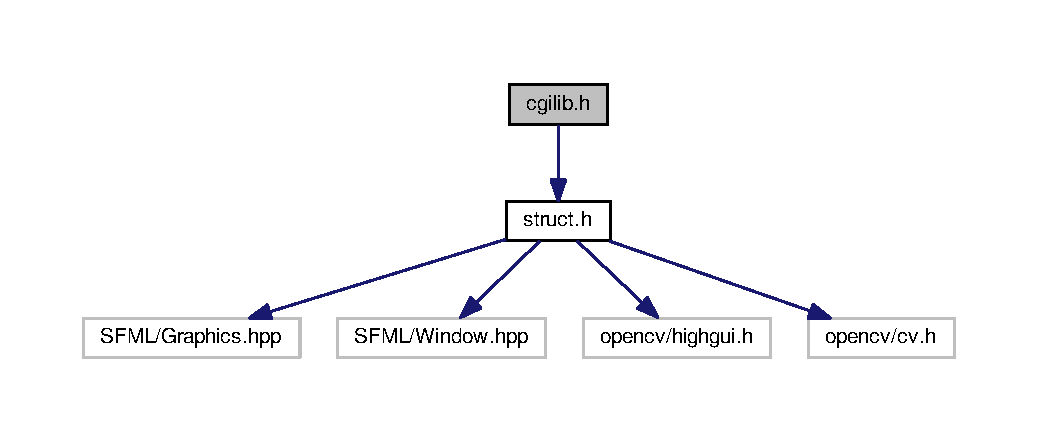
\includegraphics[width=350pt]{cgilib_8h__incl}
\end{center}
\end{figure}
This graph shows which files directly or indirectly include this file\+:
\nopagebreak
\begin{figure}[H]
\begin{center}
\leavevmode
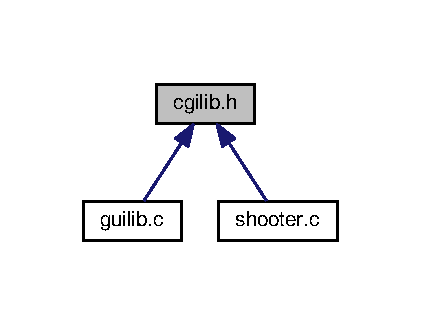
\includegraphics[width=202pt]{cgilib_8h__dep__incl}
\end{center}
\end{figure}
\subsection*{Functions}
\begin{DoxyCompactItemize}
\item 
void \hyperlink{cgilib_8h_a59601d55e89384d9c991d0a306f28f04}{laser} (Ipl\+Image $\ast$img, int frame\+Number)
\begin{DoxyCompactList}\small\item\em Fonction d\textquotesingle{}animation des lasers sur l\textquotesingle{}image. \end{DoxyCompactList}\item 
void \hyperlink{cgilib_8h_ae3d713a42a97f1b819a5b94c5bea91ae}{release\+\_\+final} (\hyperlink{struct_camera}{Camera} $\ast$cam, struct \hyperlink{struct___c_g_i}{\+\_\+\+C\+GI} $\ast$after\+Effect)
\begin{DoxyCompactList}\small\item\em Fonction de libération de la mémoire que l\textquotesingle{}on a allouée au début du programme (et pas dans la boucle infinie) \end{DoxyCompactList}\item 
void \hyperlink{cgilib_8h_a9c332fda0ae3ab452aafa58f42432a76}{release\+\_\+boucle} (struct \hyperlink{struct___c_g_i}{\+\_\+\+C\+GI} $\ast$after\+Effect, \hyperlink{struct_camera}{Camera} $\ast$cam)
\begin{DoxyCompactList}\small\item\em Fonction de libération de la mémoire que l\textquotesingle{}on a allouée dans la boucle infinie du programme. \end{DoxyCompactList}\item 
Ipl\+Image $\ast$ \hyperlink{cgilib_8h_affce441e08e063a310c74cf737ccae8c}{resize} (Ipl\+Image $\ast$src, int percentage)
\begin{DoxyCompactList}\small\item\em Fonction qui redimensionne une image en pourcentage de sa taille initiale. \end{DoxyCompactList}\item 
Ipl\+Image $\ast$ \hyperlink{cgilib_8h_a25a21584c96a36aba95f6d40245de59d}{init\+\_\+cockpit} (int i)
\item 
void \hyperlink{cgilib_8h_aef64f26cc8f7854b0cfcbf94efa105d1}{calcul\+\_\+patate} (\hyperlink{struct_patatoide}{Patatoide} $\ast$patate, \hyperlink{struct_camera}{Camera} $\ast$cam, float coeff)
\begin{DoxyCompactList}\small\item\em Fonction effectuant des calculs amenant à connaître le centre et la taille du patatoïde observé. \end{DoxyCompactList}\item 
void \hyperlink{cgilib_8h_a04d30fac7dc18ecc16cdd21f96aa16ed}{init\+\_\+mask} (struct \hyperlink{struct___c_g_i}{\+\_\+\+C\+GI} $\ast$after\+Effect)
\begin{DoxyCompactList}\small\item\em Fonction initialisant les valeurs des bornes haute et basse utilisées dans la création du mask. \end{DoxyCompactList}\item 
void \hyperlink{cgilib_8h_a47fe4ad353e7a066c4bcdc9572605c65}{create\+\_\+mask} (struct \hyperlink{struct___c_g_i}{\+\_\+\+C\+GI} $\ast$after\+Effect, int mode, int w\+\_\+resized, int h\+\_\+resized)
\begin{DoxyCompactList}\small\item\em Fonction de création du mask. \end{DoxyCompactList}\item 
int \hyperlink{cgilib_8h_a5423edb32e5bf81ad59c86966a7494c6}{init\+\_\+cam} (\hyperlink{struct_camera}{Camera} $\ast$cam)
\begin{DoxyCompactList}\small\item\em Fonction d\textquotesingle{}initialisation des différents paramètres liées à la caméra. \end{DoxyCompactList}\item 
void \hyperlink{cgilib_8h_a38a7d29cdb7a9f133a6845b22644e6ac}{insert\+\_\+image} (struct \hyperlink{struct___c_g_i}{\+\_\+\+C\+GI} $\ast$after\+Effect, \hyperlink{struct_camera}{Camera} $\ast$cam, \hyperlink{struct_patatoide}{Patatoide} $\ast$patate, int mode)
\begin{DoxyCompactList}\small\item\em Fonction d\textquotesingle{}insertion d\textquotesingle{}image plus petite dans l\textquotesingle{}image affichée. \end{DoxyCompactList}\item 
int \hyperlink{cgilib_8h_a731bf42d8f37ed38b2865dd7b06bb031}{is\+Touched} (\hyperlink{struct_patatoide}{Patatoide} patate)
\begin{DoxyCompactList}\small\item\em Fonction qui détermine si l\textquotesingle{}on a touché l\textquotesingle{}étoile ou non lors de notre tir. \end{DoxyCompactList}\end{DoxyCompactItemize}


\subsection{Detailed Description}
Ce fichier contient les prototypes des fonctions du fichier \hyperlink{cgilib_8c}{cgilib.\+c}. 

\begin{DoxyAuthor}{Author}
Elias H. 
\end{DoxyAuthor}
\begin{DoxyVersion}{Version}
1.\+0 
\end{DoxyVersion}
\begin{DoxyDate}{Date}
30 mai 2017 
\end{DoxyDate}


\subsection{Function Documentation}
\index{cgilib.\+h@{cgilib.\+h}!calcul\+\_\+patate@{calcul\+\_\+patate}}
\index{calcul\+\_\+patate@{calcul\+\_\+patate}!cgilib.\+h@{cgilib.\+h}}
\subsubsection[{\texorpdfstring{calcul\+\_\+patate(\+Patatoide $\ast$patate, Camera $\ast$cam, float coeff)}{calcul_patate(Patatoide *patate, Camera *cam, float coeff)}}]{\setlength{\rightskip}{0pt plus 5cm}void calcul\+\_\+patate (
\begin{DoxyParamCaption}
\item[{{\bf Patatoide} $\ast$}]{patate, }
\item[{{\bf Camera} $\ast$}]{cam, }
\item[{float}]{coeff}
\end{DoxyParamCaption}
)}\hypertarget{cgilib_8h_aef64f26cc8f7854b0cfcbf94efa105d1}{}\label{cgilib_8h_aef64f26cc8f7854b0cfcbf94efa105d1}


Fonction effectuant des calculs amenant à connaître le centre et la taille du patatoïde observé. 


\begin{DoxyParams}{Parameters}
{\em patate} & Structure contenant les informations sur le patatoïde. \\
\hline
{\em cam} & Structure contenant des pointeurs sur les images utilisées dans le programme. \\
\hline
{\em coeff} & Valeur choisie à 0.\+1 ajustant la variation de la taille du patatoïde pour empêcher une évolution trop brusque. \\
\hline
\end{DoxyParams}
\begin{DoxyReturn}{Returns}
void. 
\end{DoxyReturn}
\index{cgilib.\+h@{cgilib.\+h}!create\+\_\+mask@{create\+\_\+mask}}
\index{create\+\_\+mask@{create\+\_\+mask}!cgilib.\+h@{cgilib.\+h}}
\subsubsection[{\texorpdfstring{create\+\_\+mask(struct \+\_\+\+C\+G\+I $\ast$after\+Effect, int mode, int w\+\_\+resized, int h\+\_\+resized)}{create_mask(struct _CGI *afterEffect, int mode, int w_resized, int h_resized)}}]{\setlength{\rightskip}{0pt plus 5cm}void create\+\_\+mask (
\begin{DoxyParamCaption}
\item[{struct {\bf \+\_\+\+C\+GI} $\ast$}]{after\+Effect, }
\item[{int}]{mode, }
\item[{int}]{w\+\_\+resized, }
\item[{int}]{h\+\_\+resized}
\end{DoxyParamCaption}
)}\hypertarget{cgilib_8h_a47fe4ad353e7a066c4bcdc9572605c65}{}\label{cgilib_8h_a47fe4ad353e7a066c4bcdc9572605c65}


Fonction de création du mask. 


\begin{DoxyParams}{Parameters}
{\em after\+Effect} & Structure contenant le mask à créer. \\
\hline
{\em mode} & permet de choisir quel mask créer (mode = 0 pour le mask du cockpit et mode = 1 pour le mask de l\textquotesingle{}étoile de la mort). \\
\hline
{\em w\+\_\+resized} & Seulement pour le mode 1, largeur de l\textquotesingle{}image à masquer. \\
\hline
{\em h\+\_\+resized} & eulement pour le mode 1, hauteur de l\textquotesingle{}image à masquer. \\
\hline
\end{DoxyParams}
\begin{DoxyReturn}{Returns}
void. 
\end{DoxyReturn}
\index{cgilib.\+h@{cgilib.\+h}!init\+\_\+cam@{init\+\_\+cam}}
\index{init\+\_\+cam@{init\+\_\+cam}!cgilib.\+h@{cgilib.\+h}}
\subsubsection[{\texorpdfstring{init\+\_\+cam(\+Camera $\ast$cam)}{init_cam(Camera *cam)}}]{\setlength{\rightskip}{0pt plus 5cm}int init\+\_\+cam (
\begin{DoxyParamCaption}
\item[{{\bf Camera} $\ast$}]{cam}
\end{DoxyParamCaption}
)}\hypertarget{cgilib_8h_a5423edb32e5bf81ad59c86966a7494c6}{}\label{cgilib_8h_a5423edb32e5bf81ad59c86966a7494c6}


Fonction d\textquotesingle{}initialisation des différents paramètres liées à la caméra. 


\begin{DoxyParams}{Parameters}
{\em cam} & Structure contenant les variables et images à initialiser. \\
\hline
\end{DoxyParams}
\begin{DoxyReturn}{Returns}
void. 
\end{DoxyReturn}
\index{cgilib.\+h@{cgilib.\+h}!init\+\_\+cockpit@{init\+\_\+cockpit}}
\index{init\+\_\+cockpit@{init\+\_\+cockpit}!cgilib.\+h@{cgilib.\+h}}
\subsubsection[{\texorpdfstring{init\+\_\+cockpit(int i)}{init_cockpit(int i)}}]{\setlength{\rightskip}{0pt plus 5cm}Ipl\+Image$\ast$ init\+\_\+cockpit (
\begin{DoxyParamCaption}
\item[{int}]{i}
\end{DoxyParamCaption}
)}\hypertarget{cgilib_8h_a25a21584c96a36aba95f6d40245de59d}{}\label{cgilib_8h_a25a21584c96a36aba95f6d40245de59d}
\index{cgilib.\+h@{cgilib.\+h}!init\+\_\+mask@{init\+\_\+mask}}
\index{init\+\_\+mask@{init\+\_\+mask}!cgilib.\+h@{cgilib.\+h}}
\subsubsection[{\texorpdfstring{init\+\_\+mask(struct \+\_\+\+C\+G\+I $\ast$after\+Effect)}{init_mask(struct _CGI *afterEffect)}}]{\setlength{\rightskip}{0pt plus 5cm}void init\+\_\+mask (
\begin{DoxyParamCaption}
\item[{struct {\bf \+\_\+\+C\+GI} $\ast$}]{after\+Effect}
\end{DoxyParamCaption}
)}\hypertarget{cgilib_8h_a04d30fac7dc18ecc16cdd21f96aa16ed}{}\label{cgilib_8h_a04d30fac7dc18ecc16cdd21f96aa16ed}


Fonction initialisant les valeurs des bornes haute et basse utilisées dans la création du mask. 


\begin{DoxyParams}{Parameters}
{\em after\+Effect} & Structure contenant les variables de bornes haute et basse à modifier. \\
\hline
\end{DoxyParams}
\begin{DoxyReturn}{Returns}
void. 
\end{DoxyReturn}
\index{cgilib.\+h@{cgilib.\+h}!insert\+\_\+image@{insert\+\_\+image}}
\index{insert\+\_\+image@{insert\+\_\+image}!cgilib.\+h@{cgilib.\+h}}
\subsubsection[{\texorpdfstring{insert\+\_\+image(struct \+\_\+\+C\+G\+I $\ast$after\+Effect, Camera $\ast$cam, Patatoide $\ast$patate, int mode)}{insert_image(struct _CGI *afterEffect, Camera *cam, Patatoide *patate, int mode)}}]{\setlength{\rightskip}{0pt plus 5cm}void insert\+\_\+image (
\begin{DoxyParamCaption}
\item[{struct {\bf \+\_\+\+C\+GI} $\ast$}]{after\+Effect, }
\item[{{\bf Camera} $\ast$}]{cam, }
\item[{{\bf Patatoide} $\ast$}]{patate, }
\item[{int}]{mode}
\end{DoxyParamCaption}
)}\hypertarget{cgilib_8h_a38a7d29cdb7a9f133a6845b22644e6ac}{}\label{cgilib_8h_a38a7d29cdb7a9f133a6845b22644e6ac}


Fonction d\textquotesingle{}insertion d\textquotesingle{}image plus petite dans l\textquotesingle{}image affichée. 


\begin{DoxyParams}{Parameters}
{\em after\+Effect} & Structure contenant les variables et images à insérer ainsi que les mask de copie. \\
\hline
{\em cam} & Structure contenant les variables et images à modifier. \\
\hline
{\em patate} & Structure contenant les informations sur le patatoide. \\
\hline
{\em mode} & permet de choisir quelle image copier. \\
\hline
\end{DoxyParams}
\begin{DoxyReturn}{Returns}
void. 
\end{DoxyReturn}
\index{cgilib.\+h@{cgilib.\+h}!is\+Touched@{is\+Touched}}
\index{is\+Touched@{is\+Touched}!cgilib.\+h@{cgilib.\+h}}
\subsubsection[{\texorpdfstring{is\+Touched(\+Patatoide patate)}{isTouched(Patatoide patate)}}]{\setlength{\rightskip}{0pt plus 5cm}int is\+Touched (
\begin{DoxyParamCaption}
\item[{{\bf Patatoide}}]{patate}
\end{DoxyParamCaption}
)}\hypertarget{cgilib_8h_a731bf42d8f37ed38b2865dd7b06bb031}{}\label{cgilib_8h_a731bf42d8f37ed38b2865dd7b06bb031}


Fonction qui détermine si l\textquotesingle{}on a touché l\textquotesingle{}étoile ou non lors de notre tir. 


\begin{DoxyParams}{Parameters}
{\em patate} & Structure contenant les informations sur le patatoide. \\
\hline
\end{DoxyParams}
\begin{DoxyReturn}{Returns}
int 1 si l\textquotesingle{}on a touché, 0 sinon. 
\end{DoxyReturn}
\index{cgilib.\+h@{cgilib.\+h}!laser@{laser}}
\index{laser@{laser}!cgilib.\+h@{cgilib.\+h}}
\subsubsection[{\texorpdfstring{laser(\+Ipl\+Image $\ast$img, int frame\+Number)}{laser(IplImage *img, int frameNumber)}}]{\setlength{\rightskip}{0pt plus 5cm}void laser (
\begin{DoxyParamCaption}
\item[{Ipl\+Image $\ast$}]{img, }
\item[{int}]{frame\+Number}
\end{DoxyParamCaption}
)}\hypertarget{cgilib_8h_a59601d55e89384d9c991d0a306f28f04}{}\label{cgilib_8h_a59601d55e89384d9c991d0a306f28f04}


Fonction d\textquotesingle{}animation des lasers sur l\textquotesingle{}image. 


\begin{DoxyParams}{Parameters}
{\em img} & Image sur laquelle on souhaite ajouter les lasers. \\
\hline
{\em frame\+Number} & Indique à quelle frame de l\textquotesingle{}image nous sommes pour déterminer à quelle position afficher les lasers. \\
\hline
\end{DoxyParams}
\begin{DoxyReturn}{Returns}
void. 
\end{DoxyReturn}
\index{cgilib.\+h@{cgilib.\+h}!release\+\_\+boucle@{release\+\_\+boucle}}
\index{release\+\_\+boucle@{release\+\_\+boucle}!cgilib.\+h@{cgilib.\+h}}
\subsubsection[{\texorpdfstring{release\+\_\+boucle(struct \+\_\+\+C\+G\+I $\ast$after\+Effect, Camera $\ast$cam)}{release_boucle(struct _CGI *afterEffect, Camera *cam)}}]{\setlength{\rightskip}{0pt plus 5cm}void release\+\_\+boucle (
\begin{DoxyParamCaption}
\item[{struct {\bf \+\_\+\+C\+GI} $\ast$}]{after\+Effect, }
\item[{{\bf Camera} $\ast$}]{cam}
\end{DoxyParamCaption}
)}\hypertarget{cgilib_8h_a9c332fda0ae3ab452aafa58f42432a76}{}\label{cgilib_8h_a9c332fda0ae3ab452aafa58f42432a76}


Fonction de libération de la mémoire que l\textquotesingle{}on a allouée dans la boucle infinie du programme. 


\begin{DoxyParams}{Parameters}
{\em cam} & Structure contenant des pointeurs sur les mémoires à libérer \\
\hline
{\em after\+Effect} & idem que cam \\
\hline
\end{DoxyParams}
\begin{DoxyReturn}{Returns}
void. 
\end{DoxyReturn}
\index{cgilib.\+h@{cgilib.\+h}!release\+\_\+final@{release\+\_\+final}}
\index{release\+\_\+final@{release\+\_\+final}!cgilib.\+h@{cgilib.\+h}}
\subsubsection[{\texorpdfstring{release\+\_\+final(\+Camera $\ast$cam, struct \+\_\+\+C\+G\+I $\ast$after\+Effect)}{release_final(Camera *cam, struct _CGI *afterEffect)}}]{\setlength{\rightskip}{0pt plus 5cm}void release\+\_\+final (
\begin{DoxyParamCaption}
\item[{{\bf Camera} $\ast$}]{cam, }
\item[{struct {\bf \+\_\+\+C\+GI} $\ast$}]{after\+Effect}
\end{DoxyParamCaption}
)}\hypertarget{cgilib_8h_ae3d713a42a97f1b819a5b94c5bea91ae}{}\label{cgilib_8h_ae3d713a42a97f1b819a5b94c5bea91ae}


Fonction de libération de la mémoire que l\textquotesingle{}on a allouée au début du programme (et pas dans la boucle infinie) 


\begin{DoxyParams}{Parameters}
{\em cam} & Structure contenant des pointeurs sur les mémoires à libérer \\
\hline
{\em after\+Effect} & idem que cam \\
\hline
\end{DoxyParams}
\begin{DoxyReturn}{Returns}
void. 
\end{DoxyReturn}
\index{cgilib.\+h@{cgilib.\+h}!resize@{resize}}
\index{resize@{resize}!cgilib.\+h@{cgilib.\+h}}
\subsubsection[{\texorpdfstring{resize(\+Ipl\+Image $\ast$src, int percentage)}{resize(IplImage *src, int percentage)}}]{\setlength{\rightskip}{0pt plus 5cm}Ipl\+Image$\ast$ resize (
\begin{DoxyParamCaption}
\item[{Ipl\+Image $\ast$}]{src, }
\item[{int}]{percentage}
\end{DoxyParamCaption}
)}\hypertarget{cgilib_8h_affce441e08e063a310c74cf737ccae8c}{}\label{cgilib_8h_affce441e08e063a310c74cf737ccae8c}


Fonction qui redimensionne une image en pourcentage de sa taille initiale. 


\begin{DoxyParams}{Parameters}
{\em src} & Image que à redimensionner. \\
\hline
{\em percentage} & Pourcentage qui donne la taille de l\textquotesingle{}image finale par rapport à l\textquotesingle{}image initiale \\
\hline
\end{DoxyParams}
\begin{DoxyReturn}{Returns}
Ipl\+Image Image redimensionnée en fonction du pourcentage. 
\end{DoxyReturn}

\hypertarget{guilib_8c}{}\section{guilib.\+c File Reference}
\label{guilib_8c}\index{guilib.\+c@{guilib.\+c}}
{\ttfamily \#include $<$S\+F\+M\+L/\+Graphics.\+hpp$>$}\\*
{\ttfamily \#include \char`\"{}struct.\+h\char`\"{}}\\*
{\ttfamily \#include \char`\"{}cgilib.\+h\char`\"{}}\\*
Include dependency graph for guilib.\+c\+:
\nopagebreak
\begin{figure}[H]
\begin{center}
\leavevmode
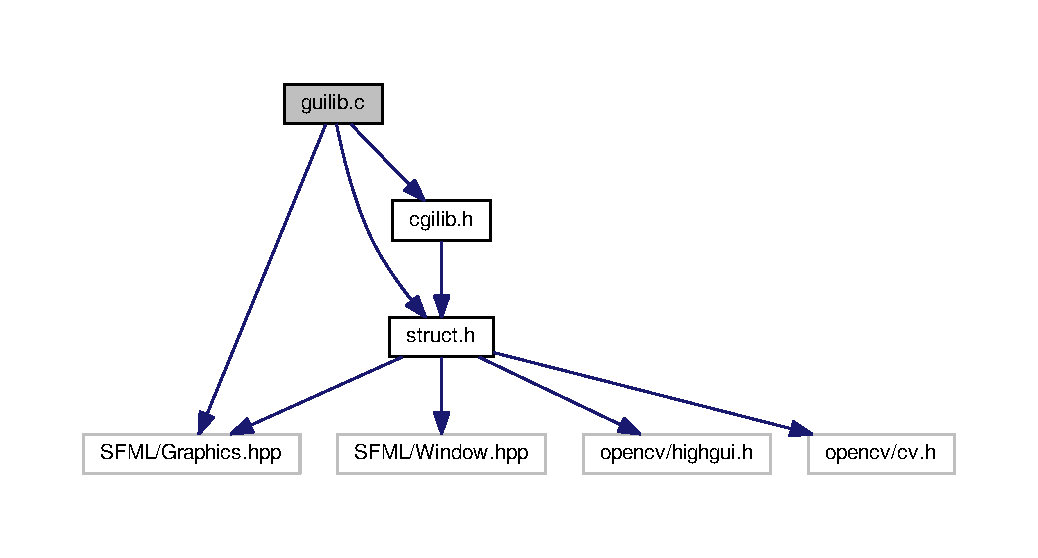
\includegraphics[width=350pt]{guilib_8c__incl}
\end{center}
\end{figure}
\subsection*{Functions}
\begin{DoxyCompactItemize}
\item 
void \hyperlink{guilib_8c_a404c6f7abeef8506547a26ba2b335a24}{init\+G\+UI} (\hyperlink{struct_8h_aac251d7a9aa683ab3e89dc84fdcdd11f}{G\+UI} $\ast$gui)
\begin{DoxyCompactList}\small\item\em initialize the gui. \end{DoxyCompactList}\item 
void \hyperlink{guilib_8c_a7c77c08733f04d6e57da2491d3d37fee}{create\+Menu} (\hyperlink{struct_8h_aac251d7a9aa683ab3e89dc84fdcdd11f}{G\+UI} $\ast$gui)
\begin{DoxyCompactList}\small\item\em initialize the gui. \end{DoxyCompactList}\item 
void \hyperlink{guilib_8c_ac4a4770a0eff0398c43245fa56a40ad4}{update\+G\+UI} (\hyperlink{struct_8h_aac251d7a9aa683ab3e89dc84fdcdd11f}{G\+UI} $\ast$gui)
\begin{DoxyCompactList}\small\item\em initialize the gui. \end{DoxyCompactList}\end{DoxyCompactItemize}


\subsection{Function Documentation}
\index{guilib.\+c@{guilib.\+c}!create\+Menu@{create\+Menu}}
\index{create\+Menu@{create\+Menu}!guilib.\+c@{guilib.\+c}}
\subsubsection[{\texorpdfstring{create\+Menu(\+G\+U\+I $\ast$gui)}{createMenu(GUI *gui)}}]{\setlength{\rightskip}{0pt plus 5cm}void create\+Menu (
\begin{DoxyParamCaption}
\item[{{\bf G\+UI} $\ast$}]{gui}
\end{DoxyParamCaption}
)}\hypertarget{guilib_8c_a7c77c08733f04d6e57da2491d3d37fee}{}\label{guilib_8c_a7c77c08733f04d6e57da2491d3d37fee}


initialize the gui. 


\begin{DoxyParams}{Parameters}
{\em G\+UI} & The gui structure. \\
\hline
\end{DoxyParams}
\index{guilib.\+c@{guilib.\+c}!init\+G\+UI@{init\+G\+UI}}
\index{init\+G\+UI@{init\+G\+UI}!guilib.\+c@{guilib.\+c}}
\subsubsection[{\texorpdfstring{init\+G\+U\+I(\+G\+U\+I $\ast$gui)}{initGUI(GUI *gui)}}]{\setlength{\rightskip}{0pt plus 5cm}void init\+G\+UI (
\begin{DoxyParamCaption}
\item[{{\bf G\+UI} $\ast$}]{gui}
\end{DoxyParamCaption}
)}\hypertarget{guilib_8c_a404c6f7abeef8506547a26ba2b335a24}{}\label{guilib_8c_a404c6f7abeef8506547a26ba2b335a24}


initialize the gui. 


\begin{DoxyParams}{Parameters}
{\em G\+UI} & The gui structure. \\
\hline
\end{DoxyParams}
\index{guilib.\+c@{guilib.\+c}!update\+G\+UI@{update\+G\+UI}}
\index{update\+G\+UI@{update\+G\+UI}!guilib.\+c@{guilib.\+c}}
\subsubsection[{\texorpdfstring{update\+G\+U\+I(\+G\+U\+I $\ast$gui)}{updateGUI(GUI *gui)}}]{\setlength{\rightskip}{0pt plus 5cm}void update\+G\+UI (
\begin{DoxyParamCaption}
\item[{{\bf G\+UI} $\ast$}]{gui}
\end{DoxyParamCaption}
)}\hypertarget{guilib_8c_ac4a4770a0eff0398c43245fa56a40ad4}{}\label{guilib_8c_ac4a4770a0eff0398c43245fa56a40ad4}


initialize the gui. 


\begin{DoxyParams}{Parameters}
{\em G\+UI} & The gui structure. \\
\hline
\end{DoxyParams}

\hypertarget{guilib_8h}{}\section{guilib.\+h File Reference}
\label{guilib_8h}\index{guilib.\+h@{guilib.\+h}}
{\ttfamily \#include \char`\"{}struct.\+h\char`\"{}}\\*
Include dependency graph for guilib.\+h\+:
\nopagebreak
\begin{figure}[H]
\begin{center}
\leavevmode
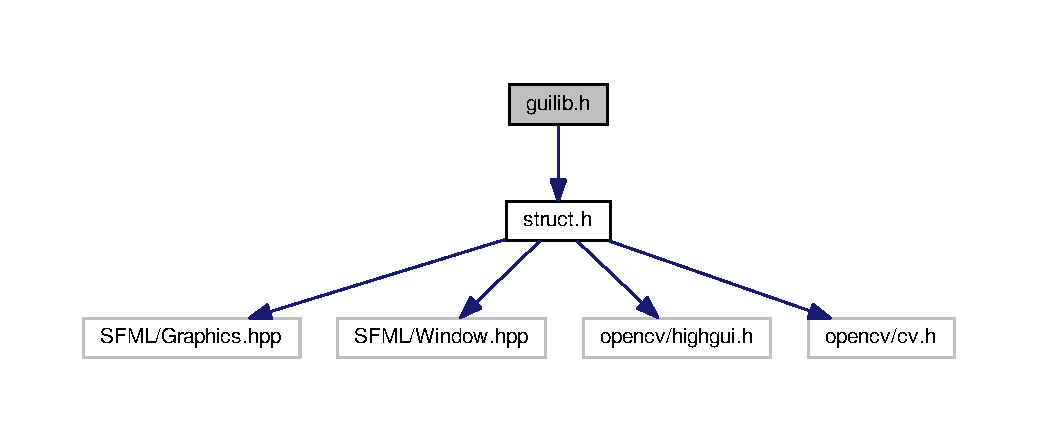
\includegraphics[width=350pt]{guilib_8h__incl}
\end{center}
\end{figure}
This graph shows which files directly or indirectly include this file\+:
\nopagebreak
\begin{figure}[H]
\begin{center}
\leavevmode
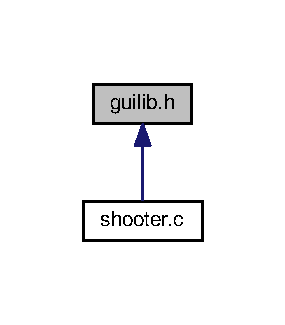
\includegraphics[width=137pt]{guilib_8h__dep__incl}
\end{center}
\end{figure}
\subsection*{Functions}
\begin{DoxyCompactItemize}
\item 
void \hyperlink{guilib_8h_a404c6f7abeef8506547a26ba2b335a24}{init\+G\+UI} (\hyperlink{struct_8h_aac251d7a9aa683ab3e89dc84fdcdd11f}{G\+UI} $\ast$gui)
\begin{DoxyCompactList}\small\item\em initialize the gui. \end{DoxyCompactList}\item 
void \hyperlink{guilib_8h_a7c77c08733f04d6e57da2491d3d37fee}{create\+Menu} (\hyperlink{struct_8h_aac251d7a9aa683ab3e89dc84fdcdd11f}{G\+UI} $\ast$gui)
\begin{DoxyCompactList}\small\item\em initialize the gui. \end{DoxyCompactList}\item 
void \hyperlink{guilib_8h_ac4a4770a0eff0398c43245fa56a40ad4}{update\+G\+UI} (\hyperlink{struct_8h_aac251d7a9aa683ab3e89dc84fdcdd11f}{G\+UI} $\ast$gui)
\begin{DoxyCompactList}\small\item\em initialize the gui. \end{DoxyCompactList}\end{DoxyCompactItemize}


\subsection{Function Documentation}
\index{guilib.\+h@{guilib.\+h}!create\+Menu@{create\+Menu}}
\index{create\+Menu@{create\+Menu}!guilib.\+h@{guilib.\+h}}
\subsubsection[{\texorpdfstring{create\+Menu(\+G\+U\+I $\ast$gui)}{createMenu(GUI *gui)}}]{\setlength{\rightskip}{0pt plus 5cm}void create\+Menu (
\begin{DoxyParamCaption}
\item[{{\bf G\+UI} $\ast$}]{gui}
\end{DoxyParamCaption}
)}\hypertarget{guilib_8h_a7c77c08733f04d6e57da2491d3d37fee}{}\label{guilib_8h_a7c77c08733f04d6e57da2491d3d37fee}


initialize the gui. 


\begin{DoxyParams}{Parameters}
{\em G\+UI} & The gui structure. \\
\hline
\end{DoxyParams}
\index{guilib.\+h@{guilib.\+h}!init\+G\+UI@{init\+G\+UI}}
\index{init\+G\+UI@{init\+G\+UI}!guilib.\+h@{guilib.\+h}}
\subsubsection[{\texorpdfstring{init\+G\+U\+I(\+G\+U\+I $\ast$gui)}{initGUI(GUI *gui)}}]{\setlength{\rightskip}{0pt plus 5cm}void init\+G\+UI (
\begin{DoxyParamCaption}
\item[{{\bf G\+UI} $\ast$}]{gui}
\end{DoxyParamCaption}
)}\hypertarget{guilib_8h_a404c6f7abeef8506547a26ba2b335a24}{}\label{guilib_8h_a404c6f7abeef8506547a26ba2b335a24}


initialize the gui. 


\begin{DoxyParams}{Parameters}
{\em G\+UI} & The gui structure. \\
\hline
\end{DoxyParams}
\index{guilib.\+h@{guilib.\+h}!update\+G\+UI@{update\+G\+UI}}
\index{update\+G\+UI@{update\+G\+UI}!guilib.\+h@{guilib.\+h}}
\subsubsection[{\texorpdfstring{update\+G\+U\+I(\+G\+U\+I $\ast$gui)}{updateGUI(GUI *gui)}}]{\setlength{\rightskip}{0pt plus 5cm}void update\+G\+UI (
\begin{DoxyParamCaption}
\item[{{\bf G\+UI} $\ast$}]{gui}
\end{DoxyParamCaption}
)}\hypertarget{guilib_8h_ac4a4770a0eff0398c43245fa56a40ad4}{}\label{guilib_8h_ac4a4770a0eff0398c43245fa56a40ad4}


initialize the gui. 


\begin{DoxyParams}{Parameters}
{\em G\+UI} & The gui structure. \\
\hline
\end{DoxyParams}

\hypertarget{joystick_8c}{}\section{joystick.\+c File Reference}
\label{joystick_8c}\index{joystick.\+c@{joystick.\+c}}
{\ttfamily \#include \char`\"{}joystick.\+h\char`\"{}}\\*
Include dependency graph for joystick.\+c\+:\nopagebreak
\begin{figure}[H]
\begin{center}
\leavevmode
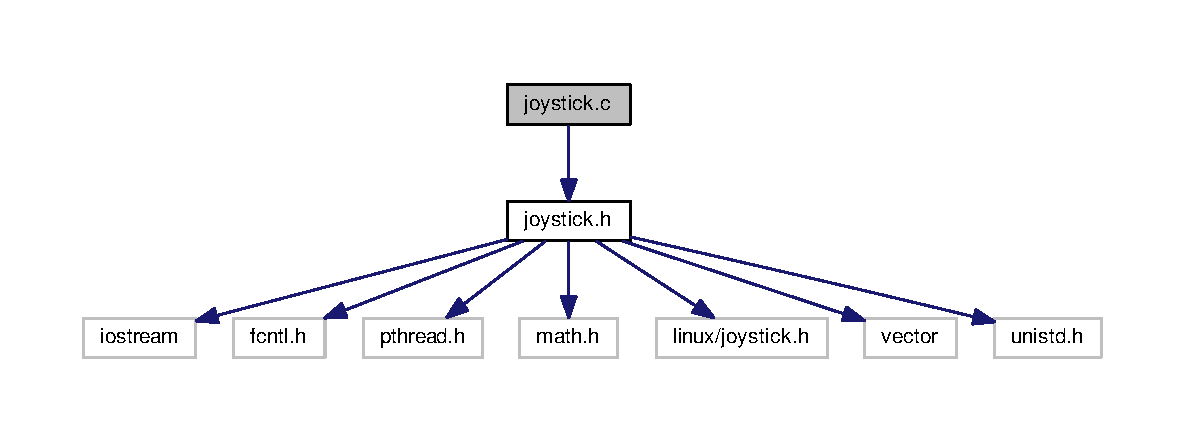
\includegraphics[width=350pt]{joystick_8c__incl}
\end{center}
\end{figure}

\hypertarget{joystick_8h}{}\section{joystick.\+h File Reference}
\label{joystick_8h}\index{joystick.\+h@{joystick.\+h}}


Ce fichier contient les prototypes des fonctions liées au joystick.  


{\ttfamily \#include $<$iostream$>$}\\*
{\ttfamily \#include $<$fcntl.\+h$>$}\\*
{\ttfamily \#include $<$pthread.\+h$>$}\\*
{\ttfamily \#include $<$math.\+h$>$}\\*
{\ttfamily \#include $<$linux/joystick.\+h$>$}\\*
{\ttfamily \#include $<$vector$>$}\\*
{\ttfamily \#include $<$unistd.\+h$>$}\\*
Include dependency graph for joystick.\+h\+:\nopagebreak
\begin{figure}[H]
\begin{center}
\leavevmode
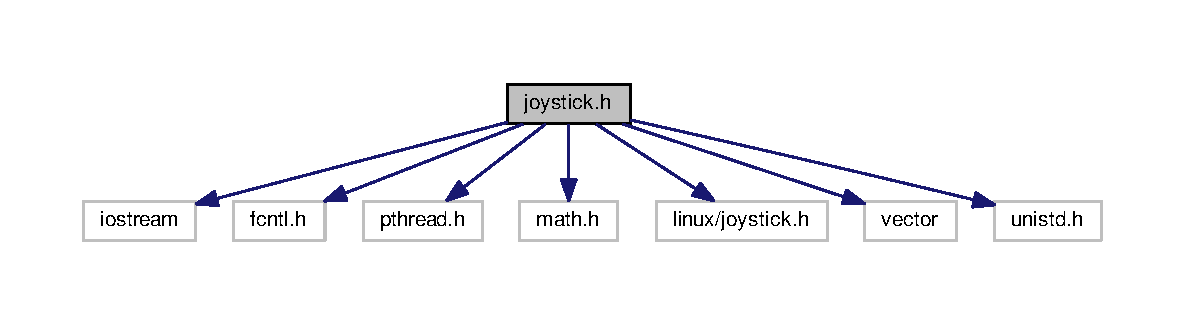
\includegraphics[width=350pt]{joystick_8h__incl}
\end{center}
\end{figure}
This graph shows which files directly or indirectly include this file\+:\nopagebreak
\begin{figure}[H]
\begin{center}
\leavevmode
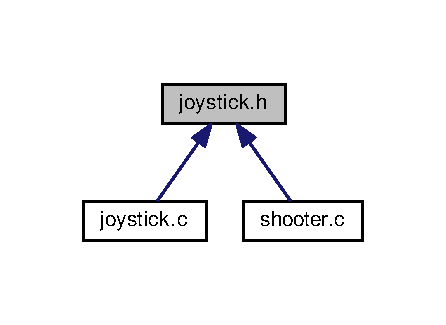
\includegraphics[width=214pt]{joystick_8h__dep__incl}
\end{center}
\end{figure}
\subsection*{Classes}
\begin{DoxyCompactItemize}
\item 
struct \hyperlink{structjoystick__position}{joystick\+\_\+position}
\item 
struct \hyperlink{structjoystick__state}{joystick\+\_\+state}
\item 
class \hyperlink{classc_joystick}{c\+Joystick}
\end{DoxyCompactItemize}
\subsection*{Macros}
\begin{DoxyCompactItemize}
\item 
\#define \hyperlink{joystick_8h_aa59cbb7e48c4f3c3dfbc694fd2869a3d}{J\+O\+Y\+S\+T\+I\+C\+K\+\_\+\+D\+EV}~\char`\"{}/dev/input/js0\char`\"{}
\end{DoxyCompactItemize}


\subsection{Detailed Description}
Ce fichier contient les prototypes des fonctions liées au joystick. 



\subsection{Macro Definition Documentation}
\index{joystick.\+h@{joystick.\+h}!J\+O\+Y\+S\+T\+I\+C\+K\+\_\+\+D\+EV@{J\+O\+Y\+S\+T\+I\+C\+K\+\_\+\+D\+EV}}
\index{J\+O\+Y\+S\+T\+I\+C\+K\+\_\+\+D\+EV@{J\+O\+Y\+S\+T\+I\+C\+K\+\_\+\+D\+EV}!joystick.\+h@{joystick.\+h}}
\subsubsection[{\texorpdfstring{J\+O\+Y\+S\+T\+I\+C\+K\+\_\+\+D\+EV}{JOYSTICK_DEV}}]{\setlength{\rightskip}{0pt plus 5cm}\#define J\+O\+Y\+S\+T\+I\+C\+K\+\_\+\+D\+EV~\char`\"{}/dev/input/js0\char`\"{}}\hypertarget{joystick_8h_aa59cbb7e48c4f3c3dfbc694fd2869a3d}{}\label{joystick_8h_aa59cbb7e48c4f3c3dfbc694fd2869a3d}

\hypertarget{mbdlib_8c}{}\section{mbdlib.\+c File Reference}
\label{mbdlib_8c}\index{mbdlib.\+c@{mbdlib.\+c}}
{\ttfamily \#include $<$stdio.\+h$>$}\\*
{\ttfamily \#include \char`\"{}mbdlib.\+h\char`\"{}}\\*
{\ttfamily \#include \char`\"{}struct.\+h\char`\"{}}\\*
{\ttfamily \#include \char`\"{}unistd.\+h\char`\"{}}\\*
{\ttfamily \#include $<$iostream$>$}\\*
Include dependency graph for mbdlib.\+c\+:\nopagebreak
\begin{figure}[H]
\begin{center}
\leavevmode
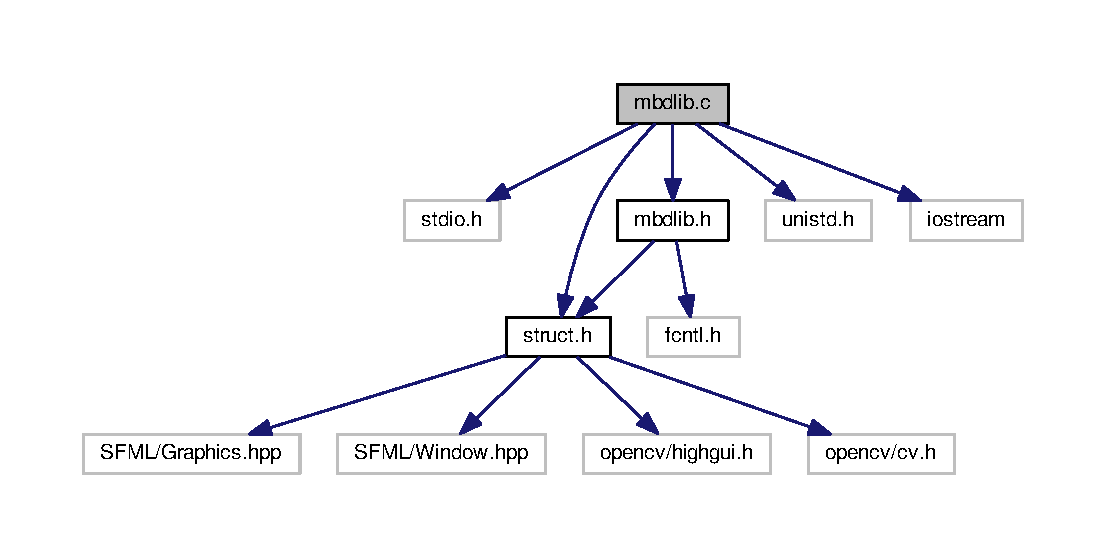
\includegraphics[width=350pt]{mbdlib_8c__incl}
\end{center}
\end{figure}
\subsection*{Functions}
\begin{DoxyCompactItemize}
\item 
void \hyperlink{mbdlib_8c_a5e6840f4bd01fcfd381e0821f034c4d1}{init\+Pantilt} (\hyperlink{struct_8h_ac76c7245da78e1fb16fa784ba8d7d52e}{Pantilt} $\ast$pnt)
\item 
int \hyperlink{mbdlib_8c_a9aaa3e4019a2a5932801e2c680dfa1f6}{move\+Pantilt} (\hyperlink{struct_8h_ac76c7245da78e1fb16fa784ba8d7d52e}{Pantilt} $\ast$pnt)
\begin{DoxyCompactList}\small\item\em Initialize the pantilt to the new position. \end{DoxyCompactList}\end{DoxyCompactItemize}


\subsection{Function Documentation}
\index{mbdlib.\+c@{mbdlib.\+c}!init\+Pantilt@{init\+Pantilt}}
\index{init\+Pantilt@{init\+Pantilt}!mbdlib.\+c@{mbdlib.\+c}}
\subsubsection[{\texorpdfstring{init\+Pantilt(\+Pantilt $\ast$pnt)}{initPantilt(Pantilt *pnt)}}]{\setlength{\rightskip}{0pt plus 5cm}void init\+Pantilt (
\begin{DoxyParamCaption}
\item[{{\bf Pantilt} $\ast$}]{pnt}
\end{DoxyParamCaption}
)}\hypertarget{mbdlib_8c_a5e6840f4bd01fcfd381e0821f034c4d1}{}\label{mbdlib_8c_a5e6840f4bd01fcfd381e0821f034c4d1}
\index{mbdlib.\+c@{mbdlib.\+c}!move\+Pantilt@{move\+Pantilt}}
\index{move\+Pantilt@{move\+Pantilt}!mbdlib.\+c@{mbdlib.\+c}}
\subsubsection[{\texorpdfstring{move\+Pantilt(\+Pantilt $\ast$pnt)}{movePantilt(Pantilt *pnt)}}]{\setlength{\rightskip}{0pt plus 5cm}void move\+Pantilt (
\begin{DoxyParamCaption}
\item[{{\bf Pantilt} $\ast$}]{pnt}
\end{DoxyParamCaption}
)}\hypertarget{mbdlib_8c_a9aaa3e4019a2a5932801e2c680dfa1f6}{}\label{mbdlib_8c_a9aaa3e4019a2a5932801e2c680dfa1f6}


Initialize the pantilt to the new position. 

Move the pantilt to the new position.


\begin{DoxyParams}{Parameters}
{\em pnt} & The pantilt structure. \\
\hline
\end{DoxyParams}

\hypertarget{mbdlib_8h}{}\section{mbdlib.\+h File Reference}
\label{mbdlib_8h}\index{mbdlib.\+h@{mbdlib.\+h}}
{\ttfamily \#include \char`\"{}struct.\+h\char`\"{}}\\*
{\ttfamily \#include $<$fcntl.\+h$>$}\\*
Include dependency graph for mbdlib.\+h\+:
\nopagebreak
\begin{figure}[H]
\begin{center}
\leavevmode
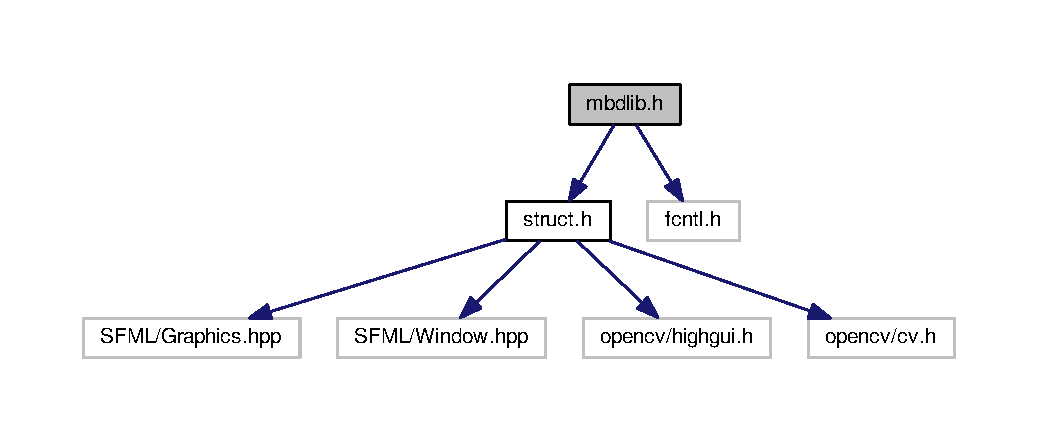
\includegraphics[width=350pt]{mbdlib_8h__incl}
\end{center}
\end{figure}
This graph shows which files directly or indirectly include this file\+:
\nopagebreak
\begin{figure}[H]
\begin{center}
\leavevmode
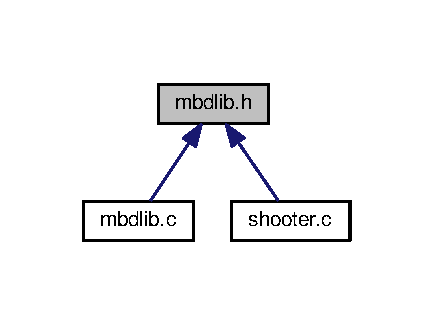
\includegraphics[width=208pt]{mbdlib_8h__dep__incl}
\end{center}
\end{figure}
\subsection*{Functions}
\begin{DoxyCompactItemize}
\item 
void \hyperlink{mbdlib_8h_a5e6840f4bd01fcfd381e0821f034c4d1}{init\+Pantilt} (\hyperlink{struct_8h_ac76c7245da78e1fb16fa784ba8d7d52e}{Pantilt} $\ast$pnt)
\item 
int \hyperlink{mbdlib_8h_adaf1617e53c25399ac540e749affb4d9}{move\+Pantilt} (\hyperlink{struct_8h_ac76c7245da78e1fb16fa784ba8d7d52e}{Pantilt} $\ast$pnt)
\begin{DoxyCompactList}\small\item\em Move the pantilt to the new position. \end{DoxyCompactList}\end{DoxyCompactItemize}


\subsection{Function Documentation}
\index{mbdlib.\+h@{mbdlib.\+h}!init\+Pantilt@{init\+Pantilt}}
\index{init\+Pantilt@{init\+Pantilt}!mbdlib.\+h@{mbdlib.\+h}}
\subsubsection[{\texorpdfstring{init\+Pantilt(\+Pantilt $\ast$pnt)}{initPantilt(Pantilt *pnt)}}]{\setlength{\rightskip}{0pt plus 5cm}void init\+Pantilt (
\begin{DoxyParamCaption}
\item[{{\bf Pantilt} $\ast$}]{pnt}
\end{DoxyParamCaption}
)}\hypertarget{mbdlib_8h_a5e6840f4bd01fcfd381e0821f034c4d1}{}\label{mbdlib_8h_a5e6840f4bd01fcfd381e0821f034c4d1}
\index{mbdlib.\+h@{mbdlib.\+h}!move\+Pantilt@{move\+Pantilt}}
\index{move\+Pantilt@{move\+Pantilt}!mbdlib.\+h@{mbdlib.\+h}}
\subsubsection[{\texorpdfstring{move\+Pantilt(\+Pantilt $\ast$pnt)}{movePantilt(Pantilt *pnt)}}]{\setlength{\rightskip}{0pt plus 5cm}int move\+Pantilt (
\begin{DoxyParamCaption}
\item[{{\bf Pantilt} $\ast$}]{pnt}
\end{DoxyParamCaption}
)}\hypertarget{mbdlib_8h_adaf1617e53c25399ac540e749affb4d9}{}\label{mbdlib_8h_adaf1617e53c25399ac540e749affb4d9}


Move the pantilt to the new position. 


\begin{DoxyParams}{Parameters}
{\em L} & The pantilt structure. \\
\hline
\end{DoxyParams}

\hypertarget{shooter_8c}{}\section{shooter.\+c File Reference}
\label{shooter_8c}\index{shooter.\+c@{shooter.\+c}}
{\ttfamily \#include $<$stdio.\+h$>$}\\*
{\ttfamily \#include $<$S\+F\+M\+L/\+Graphics.\+hpp$>$}\\*
{\ttfamily \#include $<$S\+F\+M\+L/\+Window.\+hpp$>$}\\*
{\ttfamily \#include \char`\"{}guilib.\+h\char`\"{}}\\*
{\ttfamily \#include \char`\"{}cgilib.\+h\char`\"{}}\\*
{\ttfamily \#include \char`\"{}joystick.\+h\char`\"{}}\\*
{\ttfamily \#include \char`\"{}mbdlib.\+h\char`\"{}}\\*
{\ttfamily \#include $<$iostream$>$}\\*
Include dependency graph for shooter.\+c\+:
\nopagebreak
\begin{figure}[H]
\begin{center}
\leavevmode
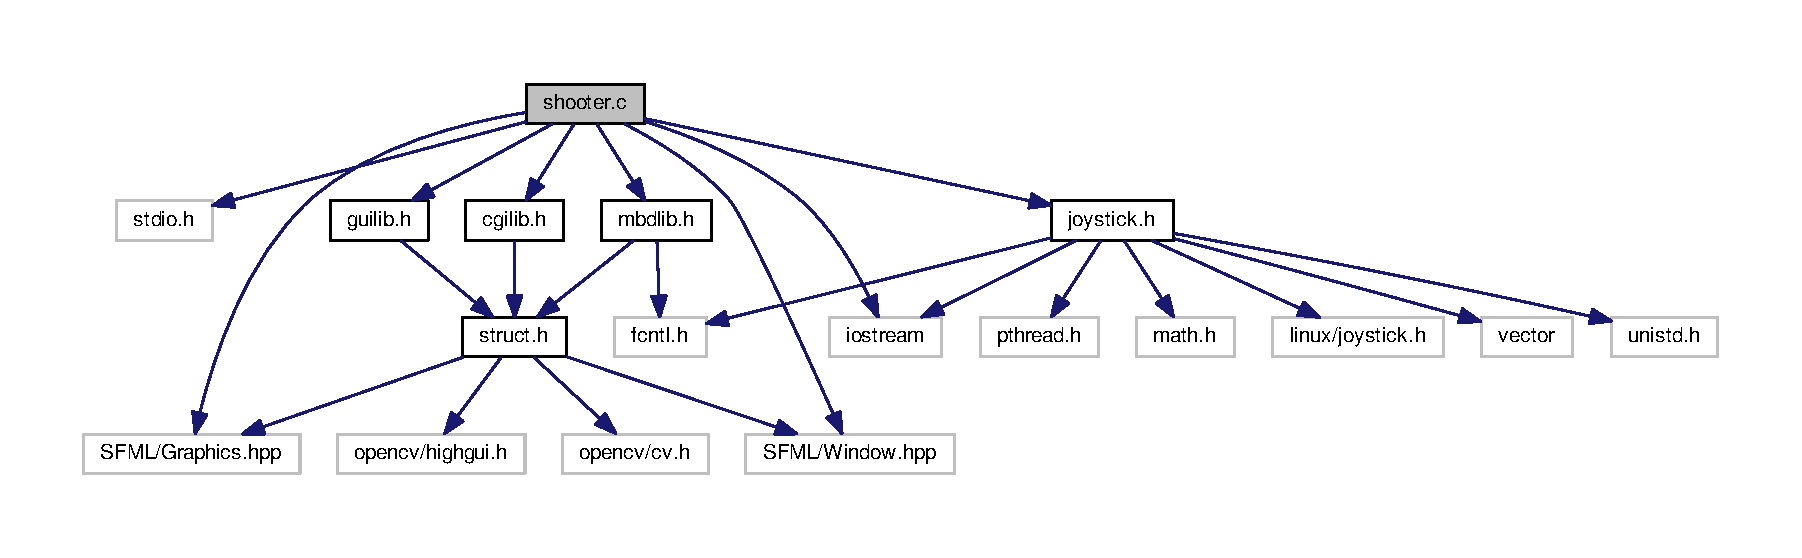
\includegraphics[width=350pt]{shooter_8c__incl}
\end{center}
\end{figure}
\subsection*{Functions}
\begin{DoxyCompactItemize}
\item 
int \hyperlink{shooter_8c_ae66f6b31b5ad750f1fe042a706a4e3d4}{main} ()
\end{DoxyCompactItemize}


\subsection{Function Documentation}
\index{shooter.\+c@{shooter.\+c}!main@{main}}
\index{main@{main}!shooter.\+c@{shooter.\+c}}
\subsubsection[{\texorpdfstring{main()}{main()}}]{\setlength{\rightskip}{0pt plus 5cm}int main (
\begin{DoxyParamCaption}
{}
\end{DoxyParamCaption}
)}\hypertarget{shooter_8c_ae66f6b31b5ad750f1fe042a706a4e3d4}{}\label{shooter_8c_ae66f6b31b5ad750f1fe042a706a4e3d4}

\hypertarget{struct_8h}{}\section{struct.\+h File Reference}
\label{struct_8h}\index{struct.\+h@{struct.\+h}}


Ce fichier regroupe les structures nécessaires à notre jeu.  


{\ttfamily \#include $<$S\+F\+M\+L/\+Graphics.\+hpp$>$}\\*
{\ttfamily \#include $<$S\+F\+M\+L/\+Window.\+hpp$>$}\\*
{\ttfamily \#include $<$opencv/highgui.\+h$>$}\\*
{\ttfamily \#include $<$opencv/cv.\+h$>$}\\*
Include dependency graph for struct.\+h\+:\nopagebreak
\begin{figure}[H]
\begin{center}
\leavevmode
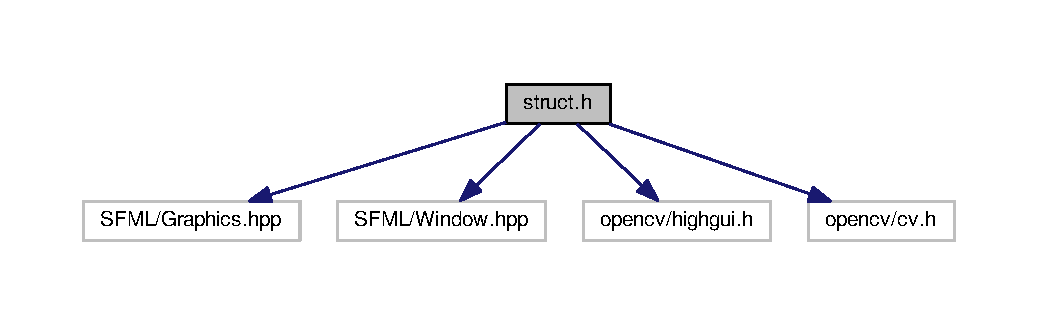
\includegraphics[width=350pt]{struct_8h__incl}
\end{center}
\end{figure}
This graph shows which files directly or indirectly include this file\+:\nopagebreak
\begin{figure}[H]
\begin{center}
\leavevmode
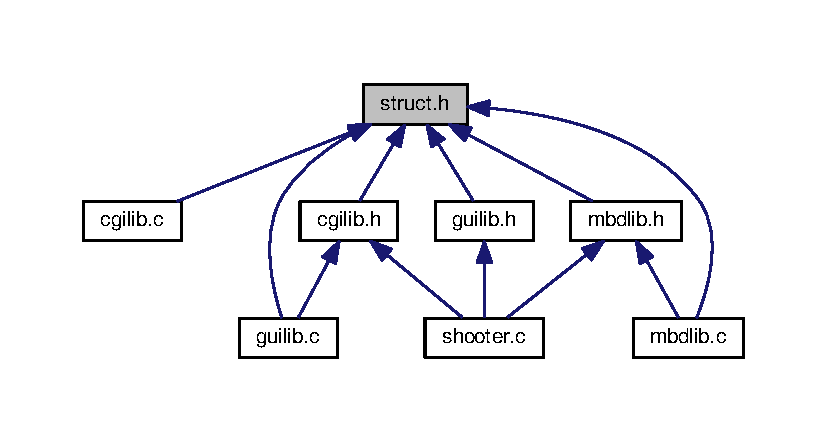
\includegraphics[width=350pt]{struct_8h__dep__incl}
\end{center}
\end{figure}
\subsection*{Classes}
\begin{DoxyCompactItemize}
\item 
struct \hyperlink{struct___g_u_i}{\+\_\+\+G\+UI}
\begin{DoxyCompactList}\small\item\em Gui est une structure composé de toutes les variable nécéssaire à linterface graphique. \end{DoxyCompactList}\item 
struct \hyperlink{struct___pantilt}{\+\_\+\+Pantilt}
\begin{DoxyCompactList}\small\item\em Regroupe les variables liées à la pantilt. \end{DoxyCompactList}\item 
struct \hyperlink{struct___camera}{\+\_\+\+Camera}
\item 
struct \hyperlink{struct___c_g_i}{\+\_\+\+C\+GI}
\item 
struct \hyperlink{struct___patatoide}{\+\_\+\+Patatoide}
\end{DoxyCompactItemize}
\subsection*{Macros}
\begin{DoxyCompactItemize}
\item 
\#define \hyperlink{struct_8h_a649b8f01fd6c0f47ff3cbddaeba63bfb}{W}~640
\item 
\#define \hyperlink{struct_8h_abec92cc72a096640b821b8cd56a02495}{H}~720
\end{DoxyCompactItemize}
\subsection*{Typedefs}
\begin{DoxyCompactItemize}
\item 
typedef struct \hyperlink{struct___g_u_i}{\+\_\+\+G\+UI} \hyperlink{struct_8h_aac251d7a9aa683ab3e89dc84fdcdd11f}{G\+UI}
\item 
typedef struct \hyperlink{struct___pantilt}{\+\_\+\+Pantilt} \hyperlink{struct_8h_ac76c7245da78e1fb16fa784ba8d7d52e}{Pantilt}
\item 
typedef struct \hyperlink{struct___camera}{\+\_\+\+Camera} \hyperlink{struct_8h_a8dc833b264f84de1d703627df0d58074}{Camera}
\item 
typedef struct \hyperlink{struct___c_g_i}{\+\_\+\+C\+GI} \hyperlink{struct_8h_ae2ad34ca93820770524c69b2f59e5a6a}{C\+GI}
\item 
typedef struct \hyperlink{struct___patatoide}{\+\_\+\+Patatoide} \hyperlink{struct_8h_af1e458f3497c6e3dcb597945dcb23e9d}{Patatoide}
\end{DoxyCompactItemize}


\subsection{Detailed Description}
Ce fichier regroupe les structures nécessaires à notre jeu. 

\begin{DoxyAuthor}{Author}
Elias H. 
\end{DoxyAuthor}
\begin{DoxyVersion}{Version}
1.\+0 
\end{DoxyVersion}
\begin{DoxyDate}{Date}
30 mai 2017 
\end{DoxyDate}


\subsection{Macro Definition Documentation}
\index{struct.\+h@{struct.\+h}!H@{H}}
\index{H@{H}!struct.\+h@{struct.\+h}}
\subsubsection[{\texorpdfstring{H}{H}}]{\setlength{\rightskip}{0pt plus 5cm}\#define H~720}\hypertarget{struct_8h_abec92cc72a096640b821b8cd56a02495}{}\label{struct_8h_abec92cc72a096640b821b8cd56a02495}
\index{struct.\+h@{struct.\+h}!W@{W}}
\index{W@{W}!struct.\+h@{struct.\+h}}
\subsubsection[{\texorpdfstring{W}{W}}]{\setlength{\rightskip}{0pt plus 5cm}\#define W~640}\hypertarget{struct_8h_a649b8f01fd6c0f47ff3cbddaeba63bfb}{}\label{struct_8h_a649b8f01fd6c0f47ff3cbddaeba63bfb}


\subsection{Typedef Documentation}
\index{struct.\+h@{struct.\+h}!Camera@{Camera}}
\index{Camera@{Camera}!struct.\+h@{struct.\+h}}
\subsubsection[{\texorpdfstring{Camera}{Camera}}]{\setlength{\rightskip}{0pt plus 5cm}typedef struct {\bf \+\_\+\+Camera}  {\bf Camera}}\hypertarget{struct_8h_a8dc833b264f84de1d703627df0d58074}{}\label{struct_8h_a8dc833b264f84de1d703627df0d58074}
\index{struct.\+h@{struct.\+h}!C\+GI@{C\+GI}}
\index{C\+GI@{C\+GI}!struct.\+h@{struct.\+h}}
\subsubsection[{\texorpdfstring{C\+GI}{CGI}}]{\setlength{\rightskip}{0pt plus 5cm}typedef struct {\bf \+\_\+\+C\+GI}  {\bf C\+GI}}\hypertarget{struct_8h_ae2ad34ca93820770524c69b2f59e5a6a}{}\label{struct_8h_ae2ad34ca93820770524c69b2f59e5a6a}
\index{struct.\+h@{struct.\+h}!G\+UI@{G\+UI}}
\index{G\+UI@{G\+UI}!struct.\+h@{struct.\+h}}
\subsubsection[{\texorpdfstring{G\+UI}{GUI}}]{\setlength{\rightskip}{0pt plus 5cm}typedef struct {\bf \+\_\+\+G\+UI} {\bf G\+UI}}\hypertarget{struct_8h_aac251d7a9aa683ab3e89dc84fdcdd11f}{}\label{struct_8h_aac251d7a9aa683ab3e89dc84fdcdd11f}
\index{struct.\+h@{struct.\+h}!Pantilt@{Pantilt}}
\index{Pantilt@{Pantilt}!struct.\+h@{struct.\+h}}
\subsubsection[{\texorpdfstring{Pantilt}{Pantilt}}]{\setlength{\rightskip}{0pt plus 5cm}typedef struct {\bf \+\_\+\+Pantilt}  {\bf Pantilt}}\hypertarget{struct_8h_ac76c7245da78e1fb16fa784ba8d7d52e}{}\label{struct_8h_ac76c7245da78e1fb16fa784ba8d7d52e}
\index{struct.\+h@{struct.\+h}!Patatoide@{Patatoide}}
\index{Patatoide@{Patatoide}!struct.\+h@{struct.\+h}}
\subsubsection[{\texorpdfstring{Patatoide}{Patatoide}}]{\setlength{\rightskip}{0pt plus 5cm}typedef struct {\bf \+\_\+\+Patatoide}  {\bf Patatoide}}\hypertarget{struct_8h_af1e458f3497c6e3dcb597945dcb23e9d}{}\label{struct_8h_af1e458f3497c6e3dcb597945dcb23e9d}

%--- End generated contents ---

% Index
\backmatter
\newpage
\phantomsection
\clearemptydoublepage
\addcontentsline{toc}{chapter}{Index}
\printindex

\end{document}
